%                                     MMMMMMMMM
%                                                                             
%  MMO    MM   MMMMMM  MMMMMMM   MM    MMMMMMMM   MMD   MM  MMMMMMM MMMMMMM   
%  MMM   MMM   MM        MM     ?MMM              MMM$  MM  MM         MM     
%  MMMM 7MMM   MM        MM     MM8M    MMMMMMM   MMMMD MM  MM         MM     
%  MM MMMMMM   MMMMMM    MM    MM  MM             MM MMDMM  MMMMMM     MM     
%  MM  MM MM   MM        MM    MMMMMM             MM  MMMM  MM         MM     
%  MM     MM   MMMMMM    MM   MM    MM            MM   MMM  MMMMMMM    MM
%
%
%          - META-NET Strategic Research Agenda | English content -
% 
% ----------------------------------------------------------------------------

\begin{document}

\maketitle

% --------------------------------------------------------------------------
\ssection*{Preface}

\null
\pagestyle{empty} 

\pagenumbering{Roman} 
\setcounter{page}{3}
\pagestyle{scrheadings}

To do: write short preface.

\bigskip As of June 2012, META-NET consists of 60 research centres in 34 European countries (p.~\pageref{metanetmembers}). META-NET is working with stakeholders from economy (software companies, technology providers and users), government agencies, research organisations, non-governmental organisations, language communities and European universities. 

\clearpage

\makefundingnotice

\cleardoublepage

% --------------------------------------------------------------------------

\ssection*{Table of Contents}

\renewcommand\contentsname{}
\tableofcontents

\addtocontents{toc}{\protect\thispagestyle{empty}\protect}
\addtocontents{toc}{{\protect\vspace*{-20mm}\protect}}

\cleardoublepage

% --------------------------------------------------------------------------
% --------------------------------------------------------------------------
% --------------------------------------------------------------------------
% Content begins here.
% --------------------------------------------------------------------------
% --------------------------------------------------------------------------
% --------------------------------------------------------------------------

\setcounter{page}{1}
\pagenumbering{arabic} 
\pagestyle{scrheadings}

\ssection[Letter from the META-NET Partners]{Letter from the META-NET Partners}

% LENGTH: One page 
% CONTENT: Traditional letter style with the signatures of six to 10 very important people from the European LT landscape (or maybe even the whole META Technology Council). See the ERTRAC SRA for a nice example on how to communicate credibility and authority.

\begin{multicols}{2}
Text
\end{multicols}

\clearpage

% --------------------------------------------------------------------------
\ssection[Executive Summary]{Executive Summary}

\begin{multicols}{2}
Many European languages run the risk of becoming victims of the digital age as they are under-represented and under-resourced online. Huge regional market opportunities remain untapped because of language barriers (Directorate-General for Translation of the European Commission, 2009). If no action is taken, speaking their mother tongue will become a severe social and economic disadvantage for many European citizens. The preservation of our linguistic and cultural diversity could become a serious economic burden for the integrated European society, but it could also turn into a strong competitive advantage, since the technologies needed for overcoming language barriers and for supporting languages in the digital age are also a key-enabling technology for the next revolution in IT. 

For decades, it has been observed and lamented that one of the last remaining frontiers of information technology is still separating our rapidly evolving technological world of mobile gadgets, PCs and Internet from the most precious and powerful asset of mankind, the human mind, the only system capable of thought, knowledge and emotion. Although we use the PC to write, the telephone to chat and the Web to search for knowledge, information technology as such has no access to the meaning, purpose and sentiment behind our trillions of written and spoken words. This is why it is unable to summarize a text, answer a question, respond to a letter and to translate reliably. In many cases it cannot even correctly pronounce a simple English sentence.   

Visionaries such as Ray Kurzweil, Marvin Minsky and Bill Gates have long predicted that this border would eventually be overcome by artificial intelligence including language understanding whereas science fiction such as the Star Trek TV series suggested attractive ways in which the increased power of the technology would change our lives. Visualized fiction more than technical prophecies surely extended the imagination of an entire generation into the right direction by establishing the fantastic concept of an invisible computer that you have a conversation with and that is able to react to the most difficult queries by correct replies and also of technology that can reliably translate any human and non-human language.

Many enterprises had started much too early to invest in language technology research and development and then lost faith again after some long periods without any tangible progress. However, during the years of apparent technological standstill, research continued to conquer new ground. The results were: a deeper theoretical understanding of language, better machine-readable dictionaries, thesauri and grammars, specialized efficient language processing algorithms, hardware with greater computing power and storage capacities, large volumes of digitized text and speech data and, most importantly, powerful new methods of statistical language processing that could exploit the language data for learning hidden regularities governing our language use.

Lately Google’s web search, Autonomy’s text analytics, Nuance’s speech technology, Google’s online translation, IBM Watson’s question answering and Apple Siri’s personal assistance have given us but a glimpse of the massive potential behind the evolving language technologies. Leading-edge industry has already reacted, but this time much more decisively. IBM, SAP, Apple, Google, Amazon, Microsoft, Nokia, Nuance, Facebook and others have started acquiring language technology enterprises left and right, among them many small promising start-up companies.  

However, all stakeholders know that today none of the industrial players possesses the needed know-how for unleashing the full potential of language technology for business and society since essential research results are still missing. Nevertheless, the speed of research keeps increasing and even small improvements can already be exploited for innovative products and services that are commercially viable.

Even if Google, Apple, Microsoft, IBM and Nuance seem to be far ahead of all competitors in language technology development, any breakthrough in one of the subareas of LT research can rapidly change this picture. New results are coming in from numerous places, among them many European universities and research organisations. Actually, because of a long history of basic-research funding and a lively LT industry of mainly sophisticated SMEs, the European LT scene is very well positioned in the race for the needed breakthroughs. To a large part, the strong European LT landscape is a direct consequence of the commercial and social interests stemming from the multilingual setting of the integrating Europe. As strange as it may sound, another advantage results from the well-known lack of pragmatism in European science. Where most of collaborative US research had abandoned computationally challenging knowledge-based or mathematically sophisticated approaches to linguistic and semantic processing, the typical European quest for truth and insight coupled with a sufficient level of funding for fundamental research became the basis for continued output of high-potential novel approaches and techniques. As a side effect, many of the pioneers in US industrial LT research and development as well as many industrial providers of technologically supported language services all over the world are of European origin.  

Would this pole position in international research together with an appropriate increase in funding be sufficient for enabling Europe to profit substantially from the next revolution in IT? We have good reason to be sceptical; after all, Europe’s track record in successful commercialization of advanced IT has not improved much since the loss of countless opportunities. Nevertheless, we strongly believe that LT offers a chance for a true success story because of several factors:

\begin{itemize}
\item A lively and diverse industrial landscape of sophisticated language technology and service providers,
\item An alliance of research communities, language industries and other stakeholders behind a shared vision and long-term research programme,
\item Large public users such as the translation and web-content services of the European Union and other national and European organizations,
\item A deep cultural and political interest in the preservation and support of all European languages in the digital society,
\item Access to immense volumes of multilingual data.
\end{itemize}

Neither politically nor economically can Europe afford to miss the boat on the foreseeable next revolution in IT because we must not leave the decisions on the degree of technological support of our languages and the cultural, social, scientific and economic exploitation of the aggregated digital contents of the world entirely to others. The danger and also threat of not taking this opportunity is real seen how our sometimes well-founded and sometimes half-hearted hesitation has put us on the international backbench in future technologies such as genetics or solar energy.

The European language technology community is dedicated to fulfilling the technology demands of the multilingual European society and to turn these needs and the emerging business opportunities into competitive advantages for our economy. To this end, we have developed this Strategic Research Agenda based on a shared vision and a careful planning involving the major stakeholder communities.

The following sections analyse the multilingual technology needs arising from the multicultural setup of our continent with its emerging single digital market. They also analyse the current state of technologies for European languages and the situation of the provider industries. 

Sections x to y summarize our shared vision of the role of language technology in the year 2020 in non-technical terms and outline three priority themes for large-scale research and innovation. 

\begin{enumerate}
\item Translation Cloud – Services for instantaneous reliable spoken and written translation among all European and major non-European languages
\item Social Intelligence and e-Participation – understanding and dialogue within and across communities of citizens, customers, clients, consumers
\item Socially Aware Interactive Assistants – analysis and synthesis of non-verbal, speech and semantic signals
\end{enumerate}
 
These thematic directions have been designed with the aim of turning the joint vision into reality and to letting Europe benefit from a technological revolution that will overcome barriers of understanding between people of different languages, between people and technology and between people and the accumulated knowledge of mankind.

The three themes build the bridge between societal needs, language technology applications, and concrete roadmaps for the organization of research, development and scientific innovation. The priority themes are contextualized in the advanced networked society and cover the main functions of language: storing, sharing and using of information and knowledge, as well as improving social interaction among humans and enabling social interaction between humans and technology. As multilingualism is at the core of European culture and becoming a global norm, one theme is devoted to overcoming language barriers.

In the final section, ways are explained in which research and innovation need to be organized, in order to achieve the targeted breakthroughs and to benefit from the immense economic opportunities they create. Core components of the sketched strategy are novel modes of large-scale collective research and interaction among the major stakeholder constituencies: research in several disciplines, technology providers, technology users, policy makers and language communities. Effective schemes for sharing resources such as data, computational language models, and generic base technologies are also an integral part of the designed strategy. Of central importance is a rapid and effectual flow of intermediate results into profitable solutions of societal impact contributing to the fertile culture of technological, social and cultural innovation targeted by the Digital Agenda and the programme Horizon 2020.
\end{multicols}

\clearpage

% --------------------------------------------------------------------------
\ssection[Introduction]{Introduction}

\begin{multicols}{2}
During the last 60 years, Europe has become a distinct political and economic structure. Culturally and linguistically it is rich and diverse. However, from Portuguese to Polish and Italian to Icelandic, everyday communication between Europe's citizens, enterprises and politicians is inevitably confronted with language barriers. The EU's institutions spend about a billion Euros a year on maintaining their policy of multilingualism, i.e., translating texts and interpreting spoken communication.

The European market for translation, interpretation, software localisation and website globalisation was estimated at €8.4 billion in 2008. Are these expenses necessary and are they even sufficient? Despite this high level of expenditure, the actual documents translated represent only a fraction of the information available to the whole population in countries with a single predominant language, such as the USA, China or Japan.

Language technology and linguistic research can make a significant contribution to removing the linguistic borders. Combined with intelligent devices and applications, language technology can help Europeans talk and do business together even if they do not speak a common language.

The economy benefits from the European single market. For example, in 2010, trade within the EU accounted for 60.3% of German exports and with other European countries totalled another 10.8%. But language barriers can bring business to a halt, especially for SMEs who do not have the financial means to reverse the situation. The only (unthinkable) alternative to a multilingual Europe would be to allow a single language to take a predominant position and replace all other languages in transnational communication. Another way to overcome language barriers is to learn foreign languages.

But given the multitude of European languages (23 official languages and 60 or more others), language learning just cannot solve the problem of cross-border communication. Without technological support such as machine translation, European linguistic diversity will be an insurmountable obstacle for the entire continent.

Language technology is a key enabling technology for sustainable, cost-effective and socially beneficial solutions to language problems. Language technologies will offer European stakeholders tremendous advantages, not only within the common European market, but also in trade relations with non-European countries, especially emerging economies. Language technology solutions will eventually serve as a unique bridge between Europe's languages.

But to develop these solutions, it is absolutely essential to first carry out a systematic analysis of the linguistic particularities of all European languages, and the current state of language technology support for them. As early as the late 1970s, the EU realised the profound relevance of language technology as a driver of European unity, and began funding its first research projects, such as EUROTRA.

After a longer period of sparse funding on the European level, the European Commission set up a department dedicated to language technology and machine translation a few years ago. Currently, the EU is supporting language technology projects such as EuroMatrix and EuroMatrix+ (since 2006) and iTranslate4 (since 2010), which use basic and applied research to generate resources for establishing high-quality solutions for all European languages.

These selective funding efforts have led to a number of valuable results. For example, the translation services of the European Commission now use the Moses open-source machine translation software, which has been mainly developed in European research projects. However, these projects never led to a concerted European effort through which the EU and its member states systematically pursue the common goal of providing technology support for all European languages. Figure~\ref{fig:languages-in-research} depicts the languages that have been studied by Language Technology resaerchers in 2010, taking into account major conferences and journals. It illustrates how technology research has focussed mainly on English followed by Chinese, German, French, and a few other bigger languages. Many European languages without any reference, e.g., Slovak, Maltese, Lithuanian, Irish, Albanian, Croatian, Macedonian, Montenegrin, Romansh, Galician, Occitain, or Frisian.

\begin{figure*}[htb]
  \colorrule{grey3}{\textwidth}{1.5pt}
  \center
  \includegraphics[width=\textwidth]{../_media/Languages-in-LT-Research}
  \caption{Languages treated in the 2010 editions of Journal of Computational Linguistics and Conferences of ACL, EMNLP and COLING (source: own research)}
  \label{fig:languages-in-research}
  \colorrule{grey3}{\textwidth}{1.5pt}
\end{figure*}

Research activities have tended to be isolated, delivering valuable results but failing to make a decisive impact on the market. Even worse, in many cases research funded in Europe eventually bore fruit outside Europe. Google and Apple have been noteworthy beneficiaries. In fact, many of the predominant actors in the field today are privately-owned for-profit enterprises based in North America.

Most of their language technology systems rely on imprecise statistical approaches that do not make use of deeper linguistic methods and knowledge. For example, sentences are often automatically translated by comparing each new sentence against thousands of sentences previously translated by humans. The quality of the output largely depends on the size and quality of the available data. While the automatic translation of simple sentences in languages with sufficient amounts of available textual data can achieve useful results, shallow statistical methods are doomed to fail in the case of languages with a much smaller body of sample data or in the case of new sentences with complex structures. Analysing the deeper structural properties of languages is the only way forward if we want to build applications that perform well across the entire range of European languages.

Europe now has a well-developed research base. Through initiatives like CLARIN and META-NET the research community is well-connected and engaged in a long term agenda that is gradually strengthening language technology's role within the European Commission. Yet at the same time, our position is worse compared to other multilingual societies. Despite fewer financial resources, countries like India (22 official languages) and South Africa (11 official languages) have set up long-term national programmes for language research and technology development.

What is missing in Europe is a lack of awareness and of political determination and courage that would take us to a leading position in this technology area through a concerted funding effort.

Drawing on the insights gained so far, today’s hybrid language technology mixing deep processing with statistical methods should be able to bridge the gap between all European languages and beyond. In the end, high-quality language technology will be a must for all of Europe's languages for supporting the political and economic unity through cultural diversity.

Language technology can help tear down existing barriers and build bridges between Europe’s languages. In the digital age, communication with people and machines, as well as the unrestricted access to the knowledge of the world should be possible for all languages.

But it will depend on the commitment of all stakeholders across science, business, governance, and society to unite their efforts for the common good.  This white paper series complements the other strategic actions taken by META-NET (see the appendix for an overview). Up-to-date information can be found on the META-NET web site: \url{http://www.meta-net.eu}.
\end{multicols}

\clearpage

% --------------------------------------------------------------------------
\ssection[Multilingual Europe: Facts, Challenges, Opportunities]{Multilingual Europe: Facts, Challenges, Opportunities}

\begin{multicols}{2}

\subsection{The Statuts of Europe's Languages in Today's Networked Society}
\label{sec:status-europes-languages}

Europe’s more than 80 languages are one of its richest and most important cultural assets, and a vital part of its unique social model.\footnote{European Commission, Multilingualism: an asset for Europe and a shared commitment, Brussels, 2008 (\url{http://ec.europa.eu/languages/news/20080918-commission-communication-on-multilingualism_en.htm}).}  While languages such as English and Spanish are likely to thrive in the emerging digital marketplace, many European languages could become marginal in a networked society. This would weaken Europe’s global standing, and run counter to the strategic goal of ensuring equal participation for every European citizen regardless of language. A recent UNESCO report on multilingualism states that languages are an essential medium for the enjoyment of fundamental rights, such as political expression, education and participation in society.\footnote{UNESCO Director-General, Intersectoral mid-term strategy on languages and multilingualism, Paris, 2007 (\url{http://unesdoc.unesco.org/images/0015/001503/150335e.pdf}).} From the very beginning, Europe had decided to keep its cultural and linguistic richness and diversity alive during the process of becoming an economic and political union. For maintaining the policy of multilingualism, the EU’s institutions spend about a billion euros a year on translating texts and interpreting spoken communication. For the entire European economies the translation costs for compliance with the laws and regulations are much higher.
 
A single European market that secures wealth and social well-being is possible, but linguistic barriers still severely limit the free flow of goods, information and services. With the increased number of EU members and the general trend towards timely trans-border interaction, everyday communication between Europe’s citizens, within business and among politicians is more and more becoming confronted with language barriers. Many Europeans find it difficult to interact with online services and participate in the digital economy. According to a recent report from the European Commission, 57\% of Internet users in Europe purchase goods and services in languages that are not their native language. (English is the most common foreign language followed by French, German and Spanish.) 55\% of users read content in a foreign language while only 35\% use another language to write e-mails or post comments on the Web.\footnote{European Commission Directorate-General Information Society and Media, Organization, User language preferences online, Flash Eurobarometer \#313, 2011.}  A few years ago, English might have been the lingua franca of the Web—the vast majority of content on the Web was in English—but the situation has now drastically changed. The amount of online content in other European (as well as Asian and Middle Eastern) languages has exploded. Already today, more than 55\% of web-based content is not in English while other estimates suggest that only 50\% of Twitter messages are in English.\footnote{\url{http://www.internetworldstats.com/stats7.htm}, \url{http://semiocast.com/downloads/Semiocast_Half_of_messages_on_Twitter_are_not_in_English_20100224.pdf}.}

The fragmentation of languages on the web has been illustrated by a study reported on the google research blog\footnote{http://googleresearch.blogspot.com/2011/07/languages-of-world-wide-web.html} (see Figure~\ref{fig:language-graph-of-the-web}). The figure displays cross-lingual links excluding the English language. It clearly shows how many European languages are practically isolated on the web.

\begin{figure*}[htb]
  \colorrule{grey3}{\textwidth}{1.5pt}
  \center
  \includegraphics[width=\textwidth]{../_media/Language-Graph}
  \caption{Language graph of the web}
  \label{fig:language-graph-of-the-web}
  \colorrule{grey3}{\textwidth}{1.5pt}
\end{figure*}

Surprisingly, this ubiquitous digital divide due to language borders has not gained much public attention; yet, it raises a very pressing question: Which European languages will thrive in the networked information and knowledge society, and which are doomed to disappear?

According to some estimates, the European market volume for translation, and interpretation, comprising software localisation and website globalisation was 5.7 billion € in 2008. The sector subtitling and dubbing was at 633 million €, language teaching at 1.6 billion €. The overall value of the European language industry was estimated € 8.4 billion in 2008 and was expected to grow by 10\% per annum.\footnote{European Commission Directorate-General for Translation, Size of the language industry in the EU, Kingston Upon Thames, 2009 (\url{http://ec.europa.eu/dgs/translation/publications/studies}).}  Yet, this existing capacity is not enough to satisfy current and future needs, e.g., with regard to translation. Already today, Google claims to translate roughly the same volume per day that all human translators on the planet translate within one year.\footnote{\url{http://googleblog.blogspot.de/2012/04/breaking-down-language-barriersix-years.html}} 

Despite of recent improvements, the quality and usability of machine translation is far from what is needed. If we rely on existing technologies, automated translation and the ability to process a variety of content in a variety of languages, a key requirement for the future Internet, will be impossible. The same argument applies to information services, document services, media industries, digital archives and language teaching. There is an urgent need for innovative technologies that help save costs while offering faster and better language services to European citizens. 

The most compelling solution for ensuring the breadth and depth of language usage in Europe tomorrow is to use appropriate technology, just as we use technology to solve our transport and energy needs among others. Still, despite of recent improvements, the quality and usability of technologies such as machine translation is far from what is needed. META-NET has conducted an analysis on the current state of the official European languages as well as other important national and regional languages in Europe with special attention to their language technology support. The result of this analysis is published in a series of white papers (Rehm and Uszkoreit 2012) showing that especially the smaller European languages already today suffer from under-representation in the digital realm. Moreover, there are tremendous deficits in technology support and significant research gaps for all languages. For example, the machine translation support for 23 out of the studied 30 languages has been evaluated as having limited quality and performance, which is an alarming result. Despite problems with translation quality, Google Translate reports to translate 100 million words every week in 200 different countries, which underpins that the need is real.\footnote{\url{http://mashable.com/2011/12/08/android-app-stats/}}  

\subsection{How can Language Technology help?}
\label{sec:how-can-language-technology-help}

One way to overcome the language barrier is to learn foreign languages. Yet without technological support, mastering the 23 official languages of the European Union and some 60 other European languages is an insurmountable obstacle for Europe’s citizens, economy, political debate, and scientific progress. The solution is to build key enabling technologies: language technologies will offer European stakeholders tremendous advantages, not only within the common European market, but also in trade relations with non-European countries, especially emerging economies. Language technology solutions will eventually serve as a unique bridge between Europe’s languages. 

Language technology (LT) is a key enabling technology for the knowledge society. LT supports humans in everyday tasks, such as writing e-mails, searching for information online or booking a flight. We benefit from language technology when we:

\begin{itemize}
\item use the spelling and grammar checking features in a word processor;
\item view product recommendations at an online shop;
\item hear the verbal instructions of a synthetic voice in a navigation system;
\item translate web pages with an online service. 
\end{itemize}

Although most language services are provided by American companies, some of them such as online translation are free of charge. The recent success of Watson, an IBM computer system that won an episode of the Jeopardy game show against human candidates, illustrates the immense potential of language technology. As Europeans, we have to ask ourselves several urgent questions:

\begin{itemize}
\item Should our communications and knowledge infrastructure be dependent upon monopolistic companies?
\item How do we respond when the language-related services that we rely upon are switched off?
\item Are we actively competing in the global landscape for research and development in language technology?
\item Can we expect third parties from other continents to solve our problems of translation and knowledge management in a way that suits our specific communicative and societal needs?
\item Can the European cultural background help shape the knowledge society by offering better, more secure, more precise, more innovative and more robust high-quality technology?
\end{itemize}

We believe that secure and innovative language technology made in Europe will significantly contribute to future European economic growth and social stability while establishing for Europe a worldwide, leading position in technology innovation, securing Europe's future as a world-wide trader and exporter of goods, services and information.

\subsection{What Societal Challenges can be Addressed Using Language Technology?}
\label{sec:what-soci-challenges}

We cannot predict exactly what the future information society will look like. But there is a strong likelihood that the revolution in communication technology is bringing people speaking different languages together in new ways. This is putting pressure on individuals to learn new languages and especially on developers to create new technology applications to ensure mutual understanding and access to shareable knowledge. In a global economic and information space, more languages, speakers and content interact more quickly with new types of media. The current popularity of social media (Wikipedia, Facebook, Twitter, YouTube, and, recently, Google+) is only the tip of the iceberg.

Many societal changes and economic trends confirm the urgent need to include substantial amounts of language technology in our European information and communication technology (ICT) infrastructure. Research and development efforts in language technology must increase to go beyond what is possible today.

\textbf{Linguistic, Commercial and Knowledge Barriers.} A report of the European Commission on cross-border online commerce in the EU clearly indicated that language barriers are economic barriers.\footnote{\url{http://ec.europa.eu/consumers/strategy/docs/com_staff_wp2009_en.pdf}}  Only 59\% of retailers can handle transactions in more than one language. Translation and localisation costs must be drastically lowered before broad participation in Europe’s single digital market can become a reality. In this regard, multilingual language technology is the key, especially for small and medium-sized enterprises (SMEs). At the same time, user expectations in the information society are increasing: 81\% of all Internet users think that websites produced in their country should also be available in other languages. 44\% of European users believe they miss interesting information because websites are not available in a language that they understand.\footnote{\url{http://ec.europa.eu/public_opinion/flash/fl_313_en.pdf}} These facts can no longer be ignored. The availability of reliable language technology can help establish a potentially vast market for information as well as consumer and entertainment goods in any language.

\begin{itemize}
\item \emph{Which type of LT can help?} Machine Translation (see Priority Theme 1), Social Intelligence (see Priority Theme 2)
\item \emph{Requirements for LT:} Robust and affordable language technology must be integrated into end-user software, such as web browsers and e-mail clients. 
\end{itemize}

\textbf{Ageing Population.} Demographic changes suggest the need for more assistive technologies, especially those that drastically improve spoken language access. An aging population requires technology that can help master everyday situations and provide proactive guidance. Such technologies could answer the question, “Where did I leave my glasses?” The economic cost of demographic changes will also mean that more health care services and support systems will be required in our homes. Ambient assisted living (AAL) technologies can greatly benefit from a personalised, spoken method of interaction that is possible due to recent developments in the field of robotics. 

\begin{itemize}
\item \emph{Which type of LT can help?} Socially Aware Interactive Assistants (see Priority Theme 3)
\item \emph{Requirements for LT:} The technology must be affordable and easy to use. The full complexity of language technology must also be hidden from users that have minimal experience using advanced technologies.
\end{itemize}

\textbf{People with Disabilities.} The way we deal with disabilities has changed dramatically in the last 20 years. We have shifted from an approach based on assistance, recovery or maintenance of functional capabilities to a goal of fully integrating individuals. The use of new technologies can help us reach the ambitious goal of achieving equal opportunities, promoting independent living and integrating persons with disabilities. Speech and language technologies already help people with disabilities participate in society. Noteworthy examples include screen readers, dictation systems and voice-activated services. In addition to the social aspect of such developments, there is a huge commercial market for such services. Approximately 10\% of Europeans have permanent disabilities, which means, there are about 50 million citizens with disabilities in the EU.

\begin{itemize}
\item \emph{Which type of LT can help?} Machine Translation (see Priority Theme 1), Interactive Assistants (see Priority Theme 3)
\item \emph{Requirements for LT:} The technology should include automatic sign language recognition; automatic summarization and translation; content simplification; and interactive virtual reality systems.
\end{itemize}

\textbf{Immigration and Integration.} According to the International Migration Report 2002 of the UN Department of Economic and Social Affairs, 56 million migrants lived in Europe in 2000.\footnote{UN Department of Economic and Social Affairs Population Division, International Migration Report 2002, New York, 2002 (\url{http://www.un.org/esa/population/publications/ittmig2002/2002ITTMIGTEXT22-11.pdf}).}  The number of migrants has grown roughly to 60 million people today. Facilitating communication, providing access to information in foreign languages and helping people learn European languages can help better integrate migrants into European society. In fact, speech and language technologies can dramatically improve the integration process. 

\begin{itemize}
\item \emph{Which type of LT can help?} Machine Translation (see Priority Theme 1), Interactive Assistants (see Priority Theme 3)
\item \emph{Requirements for LT:} The technology should offer advanced language learning tools; automatic real time subtitling; automatic and simultaneous speech-to-speech, text-to-text or speech-to-text translation; improved search engines; and automatic summarization.
\end{itemize}

\textbf{Personal Information Services and Customer Care as a Commodity.} Broadband access to information and services is commonplace, and mobile communication is daily routine for millions of Europeans. In this 24/7 economy we expect quick and reliable answers as well as engaging and timely online news broadcasts. But, information overload is common, and it limits exchange in the digital information society. Citizens, governments and industries would greatly benefit from new technologies that help get the situation back under control. Embedded and mobile applications enhanced with language technology will become personal assistants to everyone.

\begin{itemize}
\item \emph{Which type of LT can help?} Social Intelligence (see Priority Theme 2), Interactive Assistants (see Priority Theme 3)
\item \emph{Requirements for LT:} The technology should offer automatic and intelligent question-answering and automatic, personalised and trusted text and speech processing of e-mail messages, news items and other textual content to make information more relevant, timely and useful.
\end{itemize}

\textbf{Global Cooperation and Human Communication.} Companies need to address new markets where multiple languages are spoken and support multinational teams at disperse locations. Many jobs cannot be filled today because linguistic barriers exclude otherwise qualified personnel. A flexible and mobile population requires multilingual language skills. Improvements in language technology can enable richer interactions and provide more advanced video conferencing services. Future technologies like a three dimensional Internet can enable new modes of situation-based collaboration in the workplace as well as support more realistic training and education scenarios. We will soon be able to participate in virtual events as new forms of entertainment, cultural exchange and tourism. Combining multilingual language technology with 3D virtual worlds and simulations will let us experience being European in a brand new way. 

\begin{itemize}
\item \emph{Which type of LT can help?} Machine Translation (see Priority Theme 1), Social Intelligence (see Priority Theme 2), Interactive Assistants (see Priority Theme 3)
\item \emph{Requirements for LT:} The technology should offer advances such as simultaneous translation, automatic minute taking, video indexing and video searching to increase productivity.
\end{itemize}

\textbf{Preservation of Cultural Heritage and Linguistic Diversity.} According to the principles of the UN-endorsed World Summit on the Information Society, “[t]he Information Society should be founded on and stimulate respect for cultural identity, cultural and linguistic diversity.”\footnote{\url{http://www.itu.int/wsis/docs/geneva/official/dop.html}} In the past, much effort has been put in the creation of digital archives and virtual museums that should help promoting our cultural heritage. However, digitisation and digital asset management are only a first step. The amount of available information and language barriers still hinder the enjoyment and usage of our cultural treasures. Language technology can make this content accessible, e.g., through cross-lingual and multimedia search and machine translation.

Likewise, communicative skills need to be trained, especially in the light of today’s find-remix-share paradigm of social media. This is underlined by the UNESCO Information for All Programme, which seeks among others to “support the production of local content and foster the availability of indigenous knowledge through basic literacy and ICT literacy training.”\footnote{\url{http://www.unesco.org/new/en/communication-and-information/intergovernmental-programmes/information-for-all-programme-ifap/}}

\begin{itemize}
\item \emph{Which type of LT can help?} Machine Translation (see Priority Theme 1), Interactive Assistants (see Priority Theme 3)
\item \emph{Requirements for LT:} Computer assisted language learning and language technology should be embedded into didactic software such as serious games to help rescuing our linguistic knowledge and diversity.
\end{itemize}

\textbf{The Growing Role of Social Media and e-Participation.} Participation in online social media networks is a key characteristic of the early twenty-first century. Social media has a tremendous impact on practically all areas of society and life. Social media can also help us solve technical problems, research products, learn about interesting places or discover new recipes. At the same time, recent developments in North Africa demonstrate the ability of social media to bring citizens together so they can express political power. Social media will play a role in the discussion of important, future topics for Europe like a common energy strategy and a common foreign policy.

A key problem is that certain groups are becoming more and more detached from these developments. One can even speak of a broken link regarding communication cultures. This is an issue since both types of bottom-up movements sketched above are highly relevant for politicians, marketing experts, or journalists who would like to know what their customers or citizens think about their initiatives, products, or publications and to be able to react accordingly. However, it is not possible to process the sheer amount of information generated in multiple languages on social networks with manual approaches. 

\begin{itemize}
\item \emph{Which type of LT can help?} Social Intelligence and e-Participation (see Priority Theme 2)
\item \emph{Requirements for LT:} Sophisticated language technology must be able to analyse developments in real time.
\end{itemize}

\textbf{Market Awareness and Customer Acceptance.} Language technology is a key part of business and consumer software. The exact size of this market is difficult to pinpoint because language technologies are often hidden inside other, more visible products. Customer acceptance of language technology has been recently shown to be high. For example, market research by the Ford Motor Company indicates that the voice control system, Ford SYNC, is widely accepted.\footnote{Ford Motor Company, Fact Sheet: Ford SYNC Voice-Controlled Communications and Connectivity System (\url{http://media.ford.com/article_display.cfm?article_id=33358}).} 60\% of Ford vehicle owners use voice commands in their cars. Non-Ford owners report a three-fold increase in their willingness to consider Ford models while 32\% of existing customers admit that the technology played an important or critical role in their purchase decision. Language technology has a tremendous market potential.

\begin{itemize}
\item \emph{Which type of LT can help?} Machine Translation (see Priority Theme 1), Social Intelligence and e-Participation (see Priority Theme 2)
\item \emph{Requirements for LT:} Sophisticated language technology must support European companies to quickly enter this emerging market that covers many different languages.
\end{itemize}

\textbf{Single Market, Many Languages.} Support for the 23 official languages of the EU has major economic and social implications, but the political dimension is equally important. Europe currently lags behind countries such as India (22 “official” languages) and South Africa (11 national languages). Government programmes in these two countries actively foster the development of language technology for a significant number of official languages, especially for mobile devices.\footnote{India: \url{http://tdil.mit.gov.in}; South Africa: \url{http://www.meraka.org.za/nhn}} Mobile devices will become an even more important connection point between humans and information technology. Google already provides free translation services in 3,306 different language pairs (including Basque and Catalan) as well as voice input for 16 languages and speech output for 24 languages. The Apple iTunes and App Store has demonstrated how premium content and products can be marketed for free and for payment. Europe must address this global competition. 

\begin{itemize}
\item \emph{Which type of LT can help?} Machine Translation (see Priority Theme 1), Social Intelligence and e-Participation (see Priority Theme 2), Interactive Assistants (see Priority Theme 3)
\item \emph{Requirements for LT:} Support all European languages.
\end{itemize}

\textbf{Secure Europe.} The evolving information and knowledge society has improved human communication and information access, but the same communication networks also help some commit crimes like identity theft and Internet fraud. The effective persecution of illegal activities requires automatic tools that can help detect crimes and monitor offenders. 

\begin{itemize}
\item \emph{Which type of LT can help?} Machine Translation (see Priority Theme 1), Social Intelligence (see Priority Theme 2)
\item \emph{Requirements for LT:} Systems that can monitor, analyse and summarise large amounts of text, audio and video data in different languages (European and non-European) and from different sources (websites and social media).
\end{itemize}

The solutions presented above are strongly influenced by larger trends (see Section XXX), such as cloud computing, social media, mobile apps and web services. Many of these products and services are only available online. For example, limiting access to Facebook and Twitter strongly influenced the course of recent political developments of North Africa. In Europe, the idea of Social Innovation has recently gained interest as it “offers an effective approach to respond to social challenges by mobilizing people's creativity to develop solutions and make a better use of scarce resources”.\footnote{\url{http://ec.europa.eu/bepa/pdf/publications_pdf/social_innovation.pdf}} Social Innovation, which is also part of Europe’s 2020 strategy, critically relies on active involvement of citizens and interaction among them, which calls for supportive multilingual technology. 

Multilingualism has now become a global norm rather than an exception. Future 3D applications that embed information and communication technology require sophisticated language technology. Autonomous robots with language technology capabilities could potentially help in catastrophes by rescuing travellers from public transportation or by giving first aid.  Language technology can significantly contribute towards improving social inclusion. Language technology can also help us provide answers to urgent social challenges while creating genuine business opportunities.

Language technology can now automate the very processes of translation, content production, and knowledge management for all European languages. It can also empower intuitive language/speech-based interfaces for household electronics, machinery, vehicles, computers and robots. Real-world commercial and industrial applications are still in the early stages of development, yet R\&D achievements are creating a genuine window of opportunity. For example, machine translation is already reasonably accurate in specific domains, and experimental applications provide multilingual information and knowledge management as well as content production in many European languages. 

\end{multicols}

\clearpage

% --------------------------------------------------------------------------
\ssection[ICT: Current State, Major Trends, Technology Predictions]{ICT: Current State, Major Trends, Technology Predictions}

\begin{multicols}{2}

\subsection{ICT Trends}
\label{sec:ict-trends}

Networked computers are ubiquitous. They come in many different shapes and forms (desktop, laptop, mobiles, tablets, etc.) or are embedded in devices, objects, and systems (e.g. smart phones, cameras, washing machines, cars, heating systems, factories, traffic control systems). Software is usually available in multiple languages. Standardisation efforts such as the introduction of Unicode solved the problem of representing and displaying different scripts, alphabets, special characters. 

Despite all progress, we mostly cling to old metaphors, use cases and workflows: text processing, video, photo, email/letter, phone. There is no real interconnection between tools and services, there are no genuinely novel breakthrough concepts.

Mobile devices, apps, and social media are ever more reshaping how and when we communicate with one another and with the technical tools and devices we use both in business and private life. The way we interact with computers is no longer restricted to graphical user interfaces with limited functionality but it’s being extended through touch screens, dynamic interfaces, voice interfaces and dialogue systems, tactile interfaces, mobile devices. 

So far, language technology is not well integrated into end user applications and interfaces -- to the end user, spell checking seems to be the only notable exception. An exception that might indicate a trend towards more intelligent language-based interaction is illustrated by Apple’s introduction of the mobile assistant Siri in the latest iPhone. Dialogue systems, often adhering to the Voice XML standard, can be seen as one of the best developed language technology application today. Yet, dialogue systems are typically used only in restricted areas.

The web represents much of our knowledge. It emerged as a collection of static documents, but nowadays it is first and foremost a collection of systems and databases that can be queried through APIs, and applications such as Google Mail, Google Calendar, Facebook, eBay, Amazon. Many people only need one interface application on their computers: a web browser. Others use netbooks whose operating system more or less is the browser (Chromium OS). Behind the scenes, there is already a considerable amount of language technology incorporated in web applications such as search engines, dialogue systems, or machine translation services.

Hardware

\begin{itemize}
\item From clumsy desktop computers to the laptop to ultra-portable lightweight machines. Nowadays, the hardware landscape is even broader (mobiles, smart phones, tablets, wifi-enabled radios, television sets, scales, cameras etc.).
\item We’re no longer producing software for the desktop computer or laptop market only. Instead, there is a huge diversity when it comes to how and where computers or embedded systems (or web services or APIs etc.) are used. The most recent game changer was the concept of app stores which enable the user to purchase software with just a few clicks or taps. Part of the next game changer will be in-app purchases: you download the basic app for free and buy add-ons or special features within the app using a click or tap of the finger (example: machine translation app for the iPhone; the basic tool is available for free, specific language pairs cost you extra).
\item Personal computer hardware: 
  \begin{itemize}
  \item Desktops and laptops
  \item Netbooks, two flavours: (a) ordinary OS; (b) browser as OS (Chromium OS)
  \item Tablet computers: iPad (own, proprietary, novel OS; latest iPad: extremely HD screen)
  \item Smartphones: iPhones (own, proprietary, novel OS), Blackberrys etc.
  \item (N.B. the static landline phone seems to be destined to die a quick death soon)
  \item Specialised phones: satellite phone, emergency phone (for the elderly, for children)
  \item E-book-readers (Kindle, iPad)
  \item Music and media players: iPod etc.
  \end{itemize}
\item Household:
  \begin{itemize}
  \item Household appliances: washing machine, fridge, coffee machine, Roomba etc.
  \item Household, entertainment: TV, projectors, radio (Logitech Squeezebox etc.)
  \item Consoles: PS3, Wii, Xbox
  \item Portable consoles: PSP, Nintendo DS, iPod Touch, iPhone
  \item Cars, boats, planes (dashboard electronics, navigation systems)
  \item Special interest devices (with a specific firmware, usually updatable): GPS handsets, pulse meter, wifi scales (Withings), blood pressure measuring
  \end{itemize}
\item Future: Ambient technology
\item Huge data centres (Google, Apple, Amazon etc.), cloud computing, peer-to-peer networks (cloud storage), high-performance number crunchers and servers
\item (N.B. The EC pushed for standard mobile phone chargers – this is just the beginning, we need more standards along multiple additional dimensions)
\item Game changers: iPhone, iPad; the app ecosystem concept has radically changed everything
\end{itemize}

Software

\begin{itemize}
\item Direct Communication: E-Mail; Instant messaging, chat, Whatsapp; Video chat (Skype, Facetime, Google+ Hangouts etc.)
\item Indirect Communication: Social networks: twitter, Facebook, XING, LinkedIn; Social media: Blogs, twitter, youtube
\item Classic Office Software: Word processing, Presentations, Spreadsheets (from MS Office to iWork to Google Documents), nowadays also on the iPhone and on the iPad
\item Search and Information Services: Google, Google Books, Google News, Digital Libraries etc.
\item E-Commerce: Online shops (Amazon, eBay), online reservation services (Expedia, Opodo, HRS), online booking services (Expedia, Opodo, HRS, Eventim), online banking, online stock
\item Personal Information Management: Address and contacts database (tightly coupled with email, see Google Contacts, Apple AddressBook, Mobile Me and mobile phones), calendars (Google Calendar, iCal), to do list managers and other productivity applications
\item Media: Personal media, highly connected to social networks: photos (iPhoto, instagram, hipstamatic, flickr, Facebook, Google+), movies (iMovie, youtube etc.); User Generated and Collaboratively Generated Content: Videos, photos, texts, articles, presentations etc. (youtube, flickr, tumblr, Wikipedia); Crowd sourcing: Amazon Mechanical Turk etc.; Entertainment and information: Music (iTunes), TV shows/programmes (iTunes), Movies (iTunes), DVD, BlueRay, CD, on demand (YouTube, BBC iPlayer, ARD Mediathek), Podcasts, Video Podcasts, E-Books (Kindle, Sony E-Reader, WeTab, iPad/iBooks), E-Magazines (subscription of e-magazines on iPad; one could think of automatic translation of articles) etc.
\item Games: Online flash games (free, for a fee); location-based; multi-player (millions of users, see WoW); casual games on mobile devices; games for a good cause (big trend)
\item Location-based services: Both on the desktop and especially on the mobile: Maps (Bing Maps, Google Maps, Google Earth), recommendations, route planning; practically everybody is carrying around a GPS receiver nowadays (navigation system, mobile phone, tablet etc.).
\item Language-related software and applications: Spell- and grammar checking in word processors; nowadays also integrated in operating systems such as MacOS X.; Online translators, lexicons, dictionaries; Only just now taking off: speech recognition and dictation software (Siri).
\item Business side of software: E-Learning, Information Services, CMS, CRM (Salesforce etc.), Market studies (trend analysis and opinion mining), Business intelligence, Standard business applications (SAP etc.), B2B vs. B2C, Call centres, business letter/email communication with partners, colleagues, customers etc. in other countries.
\end{itemize}

% ●	Build a nice table (but, then, this table would fall into the “stating the obvious” category): 
% ○	Rows are software categories, columns are the umbrella topics of the Vision Groups, i.e., Language, Information/Semantics/Metadata, Media, Interaction/Interactive Services
% ○	In the table, highlight the relationships between the categories and the three columns
% ○	One possible line of argumentation: “Every single piece of software has to do with language, information, interaction!”
% ○	(There is a nice table in an old version of our Vision Document that we could re-use here.)
% ●	Figure: Language (at the top):
% ○	Information (2nd level)
% ■	Monolingual, crosslingual (multiple?), multilingual/translingual
% ○	Interaction (2nd level)
% ■	Monolingual, crosslingual (multiple?), multilingual/translingual

\begin{itemize}
\item Bottom line: (a) It’s all about language, language is the common denominator of software. (b) Communication and interaction, being able to do business (in the office, at home, on the go). (c) In addition to language it’s also all about information, especially structured information (important link to XML, Semantic Web, Linked Open Data, Web Services etc.).
\item The breakthrough and widespread use of UMTS/3G/LTE networks, smartphones and cheap ADSL lines is responsible for the fact that we’re always on(line). Now it’s our job as LT experts to realise the breakthrough that language is no longer a barrier. We need high performance, robust machine translation and related language services everywhere, at a click.
\item Tearing down language barriers using robust, high-quality, high-performance LT could be and will be the next game changer. Machines will be able to master human languages, they will be able to talk.
\item There is a huge window of opportunity now for consumer-oriented Language Technology: mobile devices are fast enough and come with enough computing power, memory and also usually a direct internet connection (via 3G/UMTS/LTE); they have a camera and are always on; it’s easy to buy apps or add-ons (in-app purchasing). This is a huge playground for entrepreneurs and startups, there are many opportunities.
\end{itemize}

\subsection{Current State}
\label{sec:current-state}

% FIXME: Diese Tabelle ist wenig aussagekräftig.

% \begin{table}[htbp]
%   \centering
%   \begin{tabular}{p{20mm}p{20mm}p{20mm}p{20mm}p{20mm}p{20mm}}
%     & 1990 & 1995 & 2005 & 2010 & Future \\
% Internet and Web & & Web 1.0, dial-up & Wifi, ADSL & Web 2.0, mobile web & Selected megatrends: Social and local apps; Online-only content and services; Paid content/services; Personalisation; Connectivity, ubiquity (Internet of Things, Cloud Computing); Web 3.0. Major Problems: Language barriers; Digital illiteracy; Cutting edge technologies inaccessible or not interoperable; Trust; etc. \\
% Hardware & Desktop PCs & & Laptops & Smart phones, eBooks, tablets, Navigators, gaming consoles, ultra lightweight devices (MacBook Air etc.) etc. & \\
% Software & Word & Netscape, Outlook, Powerpoint, Excel & Skype, Firefox, RealPlayer & Apps on the Web and mobile devices, specialised apps, casual games, audio and video on the web \\
% Applications & Word processing & Typesetting, image processing, email, web browsing & Telephonhy, audio and video playback & Social networks, local services, sharing (flickr, youtube), online content (music) \\
% Business Applications & Databases & Accounting, warehousing & Content management, customer relationship management & E-commerce & \\
% Language Technology Applications & Spell checking & Basic keyword search on the web & Rudimentary grammar checking, voice recognition, call centre applications & Rudimentary machine translation & Goal: tackle the problems above with innovative, human-centric Language Technology \\
%   \end{tabular}
%   \caption{Current State of ICT}
%   \label{tab:current-state}
% \end{table}

\subsection{Major Trends}
\label{sec:major-trends}

%● LENGTH: About 1.5 pages
%● CONTENT: Apparent trends and megatrends; further changes needed; very general level (see above for lots of content ideas). In this section the NEM people have things like “media becomes ubiquitous”, “switch mindset from technical terms to media terms”, “media becomes networkable”, “fusion of transport technologies”, “seamless and intuitive service handover between devices and environments”, “making content searchable”, “context-aware environment”, “creation of media communities”, “trust and privacy” etc.
%● What are the technology trends and early developments in research that will eventually be relevant for LT?
%● Mention iTranslate4.eu

Important trends and mega-trends:

Internet

\begin{itemize}
\item Internet, networks, cloud computing
\item Social media (convergence of digital identities; business-self and private-self)
\item Social media will change everything (in 2010 Facebook overtook Google as the most visited websites in the USA)
\item E-democracy (Wikileaks), e-government, e-communication, e-commerce
\item Location-based services and mobile devices
\item Soon (around 2012), households won’t have ADSL lines anymore. They will use mobile 3G/UMTS and LTE (20 MBit/s downlink) networks exclusively.
\item Still: information overload (although Google helps; web search is a solved problem or is conceived as a solved problem)
\item Vast availability of any kind of information (texts, media, blogs, discussions, films, movies, tv programmes, twitter etc.)
\item Exchanging and distributing personal/private data (photos, videos, music, films) will become easier.
\item Semantic Web, Linked Data, intelligent systems
\item New business models: iTunes App Store, in-app purchases
\end{itemize}

People

\begin{itemize}
\item Always-on (smartphones, iPhone, iPad, Android, apps)
\item The way people communicate, especially using ICT, is currently being redefined completely.
\item Convergence of digital identities
\item E-mail, twitter, social networks, digital photos etc. is mainstream (across all age groups)
\item Catchy phrase: “faces and places” (see Facebook Places, Foursquare, Checkins etc.)
\item Features such as “find your friends” (or find new friends or find someone you share a common interest with) on a map will be everywhere and securely available.
\end{itemize}

Software and hardware

\begin{itemize}
\item Completely new devices: iPad (also mobile)
\item Seamless integration of mobile devices into the hardware landscape at home (including very simple file transfer, including applications; Air Play etc.); in a few years there won’t be a real need for desktop or laptop computers anymore; mobile phones and tablet computers will rule the living room (desktops and laptops as power horses only).
\item Seamless transfer of files, data, applications around different mobile devices; file formats and resolutions will automatically rearrange and adapt (between mobile; tv; large HD display; video projector etc.; in the meantime Apple introuced iCloud which does all this and more). This will be the end of the desktop computer as we know it.
\item Mobile devices, smaller devices, no-display/headless/embedded devices (household appliances such as fridge, radio, tv, hoover, scales are already available with wifi and embedded systems; next up: coffee machine, electric toothbrush, lamps etc.)
\item Very big trend to voice/speech-based systems
\item Faster networks, better voice quality, video calling (see Apple’s Facetime, Skype video calls, Google+ Hangouts)
\item Faster phones with more memory and 3D-capable displays
\item Mobile phone as a payment device using NFC (Near Field Communication)
\item Interoperability of services and applications and hardware (take a photo using your mobile phone, post to flickr, Facebook, twitter; Withings wifi scale talks to fitness/running app Runkeeper via a web service)
\item Less local applications on the hard drive; more online services and cloud computing; more specialised and niche apps.
\item Trend to very simple and easy to use user interfaces and operating systems (iOS, iPhone, iPad), usability is key.
\end{itemize}

Summary of predicted changes

\begin{itemize}
\item IT services will be ubiquitous, available wherever and whenever needed
\item IT as experienced by the user will be services that combine widely distributed resources (computing, storage, software, data)
\item IT will adapt to the location, situation and needs of the end user (Emotions, habits, goals)
\item IT services will utilize a gigantic digital model of our world consisting of interlinked and overlapping components
\item Human language functionality will be an integral part of IT
\end{itemize}

\subsection{Linked Data, Open Data, Big Data}
\label{sec:linked-data-open}

Data is seen as one of the main topics of the near future. At the European Data Forum 2012 and several other occasions the “data challenge” (big data, open data, linked data and the data value chain) is seen as one of the main themes for future developments in information technology. Language technology and the research priority themes described later in this document have a strong relation to the data challenge, both as contributors and as beneficiaries. On the one hand, language technology helps to exploit the immense volumes of data that cannot be harnessed by the proven technologies of database and knowledge base technology, i.e., the wealth of information and knowledge encoded in texts. It can extract relevant information from these texts and make them accessible as structured data for automatic processing. On the other hand, language technology will be able to analyse and interpret language data much better if it can use the growing volume of available structured data as background knowledge. 

As most of humankinds knowledge, reflection, communication and planning is encoded in human language, making these data an integral part the growing data universe is the ultimate challenge for the “big data movement.”  Interpreting and interlinking textual knowledge with the linked data world will help in the process of extracting new knowledge from the masses of newly produced structured data. 

The translation cloud will benefit from data available across languages. The translation technologies being developed will also help to address data challenges, like building and cleaning data sets that span across languages or building links between existing data sets within a given or between several languages. Multilingual access is an important requirement for a European vision of eGovernment services and e-Participation in general. On one hand, language technology can make use of open, governmental data that is being developed in portals like data.gov.uk or within the upcoming European data portal. On the other hand, the enhancement of language technologies is inevitable for realizing multilingual access to public sector data for all European citizens: the sheer amount of data and language barriers between data sets are obstacles that only can be removed with technologies in the realm of, e.g., machine translation, cross-lingual information access and information extraction. Finally,  one application scenario of socially aware interactive assistants will be multilingual virtual meetings and conferences that make use of shared data sets. These data sets will provide information about individuals, organizations, settings of interactions etc.

The creation of the data sets for social interaction is a challenge in terms of privacy and re-usage of data. This leads to various open issues that need to be resolved both for the data challenge in general and for language technologies generating and consuming data:

\begin{itemize}
\item Is there a need for a public infrastructure for data sets versus a private infrastructure, having implications with regards to re-usage of data sets, licensing schemes, privacy etc.?
\item Provenance information of data sets with regards to trustworthiness, data quality, the privacy and re-usage aspects mentioned above needs to be provided as part of the whole data value chain.
\item In the realm of language technologies and localization, a huge amount of data has been developed that is crucial for processes like data cleaning and creation of (cross-lingual) links: terminological or lexical data, translation memories, and language resources in general. These data sets need to be made available in data formats and underlying, currently quite diverse models that are crucial for the data challenge, e.g. Semantic Web based technologies.
\item Areas like eGovernment focus on processing of quite specific types of data sets, e.g. financial records with many intra European differences. Language technologies need to be made ready-to-use beyond general textual input or output. This will foster their application for a great variety of data sets, and assure that they will become part of the related workflows for data creation and consumption.
\end{itemize}

With support from the 7th framework program, the data and the LT community already have started building bridges in projects and infrastructures like dbpedia, Monnet, Wikidata and META-SHARE. We are in a good position to strengthen these relations and to assure the long-term availability of data for the European multilingual information society.

\subsection{Cloud and Sky Computing}
\label{sec:cloud-sky-computing}

A major megatrend in IT is known as cloud computing.  An increasing proportion of IT solutions is offered through the Internet, expert forecasts predict that this proportion will rapidly increase.  Computing my be offered on different levels of abstraction ranging from “Infrastructures as a Service” (IaaS) via “Platforms as a Service” (PaaS) to the powerful concept of providing any suitable software product as an Internet service (Software as a Service – SaaS). Especially the latter concept has far-reaching, mainly beneficial, implications for distribution, support, customization, maintenance and pricing. It also opens new opportunities for software evolution by emerging dynamic schemes of integration, evaluation, adaptation and scaling. A well-known example is the Google Docs online suite of office applications. In language technology an increasing number of solutions are already offered as free or commercial web services, among them machine translation, language checking and text-to-speech conversion.

A special challenge for cloud computing is the need for trust. Since the services are rendered outside their sphere of control, customers demand sufficient safeguards securing performance, data protection, and persistence. Large European users of translation technology do not send their corporate language data to the exiting large online translation services because the service providers do not offer such mechanisms. The situation is even more severe for business intelligence applications where the confidentiality of the collected information can be mission critical for the relevant planning and decision processes.  

The most far-reaching and promising development within the cloud computing trend is the inter-cloud or sky computing paradigm.  Although the cloud metaphor originated from the widely used graphical icon for the Internet symbolizing the entire global network outside the user’s computer, soon the term became applied to any individual computing service provided on the Internet.  

Sky computing extends the powerful notion of cloud computing beyond its original meaning.  The term sky computing was coined for a setup in which clouds are combined into complex services, environments with workflows realizing functionalities that exceed the capabilities of the individual services.
A new line of research and development is dedicated to the creation of sky computing platforms that permit such integration. 

Language technologies are prime candidates for sky computing setups since they are often a component of complex applications such as services supporting knowledge discovery, business intelligence or text production. Taken into account the large number of languages, language variants and subject domains, a sky computing setup can provide a much larger number of language and task specific workflows through service composition than a traditional software product. Moreover, small and medium technology enterprises will be able much more easily to enter the market, stay on the market and improve their services without having to cast all demanded service combinations into their product family or into a range of bilateral OEM partnerships.
\end{multicols}

\ssection[Language Technology: State, Limitations, Potential]{Language Technology: State, Limitations, Potential}

\begin{multicols}{2}

\subsection{What is the current state of Europe’s Language Technology?}
\label{sec:what-current-state}

Answering such a global question is notoriously difficult. Of course, partial answers exist in terms of business figures, scientific challenges on technology, results from educational studies, etc. However, to date, nobody had collected these indicators and provided comparable reports for a substantial number of European languages. In order to find a comprehensive answer, META-NET has used its joined forces and produced a White Paper Series describing the current state of language technology support for 30 different European languages. The White Papers are currently being produced with a scientific publishing house (Rehm, Uszkoreit, 2012). Language White Papers were written for the following 30 European languages (including all 23 EU languages): Basque, Bulgarian, Catalan, Croatian, Czech, Danish, Dutch, English, Estonian, Finnish, French, Galician, German, Greek, Hungarian, Icelandic, Irish, Italian, Latvian, Lithuanian, Maltese, Norwegian, Polish, Portuguese, Romanian, Serbian, Slovak, Slovene, Spanish, and Swedish.

The current state of LT support varies considerably from one language community to another. In order to compare the situation between languages, the Language White Papers introduce an evaluation based on two sample application areas (machine translation and speech processing) and one underlying technology (text analysis) as well as basic resources needed for building LT applications. LT support for the languages was categorised using a five-point scale (1. excellent support; 2. good support; 3. moderate support; 4. fragmentary support; 5. weak or no support) and measured according to the following key criteria:

\textbf{Speech Processing:} quality of existing speech recognition and synthesis technologies, coverage of domains, number and size of existing speech corpora, amount and variety of available speech-based applications.

\textbf{Machine Translation:} quality of existing MT technologies, number of language pairs covered, coverage of linguistic phenomena and domains, quality and size of existing parallel corpora, amount and variety of available MT applications.

\textbf{Text Analysis:} quality and coverage of existing text analysis technologies (morphology, syntax, semantics), coverage of linguistic phenomena and domains, amount and variety of available applications, quality and size of existing (annotated) text corpora, quality and coverage of existing lexical resources (e.g., WordNet) and grammars.

\textbf{Resources:} quality and size of existing text corpora, speech corpora and parallel corpora, quality and coverage of existing lexical resources and grammars.

The in total more than 160 contributing authors to the Language White Papers prepared an initial language-specific assessment of LT support using an approach in which ca. 25 different applications, tools and resources were assessed along seven different axes and criteria. Later on, the 30 individual and language-specific matrices were condensed in multiple iterations in order to arrive at a single score per language and area. Figures~\ref{fig:speech_cluster_en} to~\ref{fig:resources_cluster_en} show that there are dramatic differences in language technology support between the various European languages and technology areas. For all LT areas, English is ahead of any other language but even support for English is far from being perfect. While there are good quality software and resources available for some languages and application areas, others, usually smaller languages, have substantial gaps. Many languages lack basic technologies for text analysis and essential resources. Others have basic tools and resources but the implementation of, for example, semantic methods is still far away. Therefore, a large-scale effort is needed to attain the ambitious goal of providing high-quality language technology support for all European languages, for example through high quality machine translation.

In the 	Language White Papers, the interested reader will find a detailed assessment of LT performance per language. For space limitations, we do not repeat the results here. What is obvious is that no language, not even English, gets the technological support it deserves. The number of badly supported and under-resourced languages is unacceptable if we do not wan to give up the principles of solidarity and subsidiarity in Europe.

\subsection{Language Technology: Industry and Business Potential}
\label{sec:lang-techn-industry}

% [FIXME: Insert input from LTInnovate?], e.g., but not limited to topics: 
% ●	The whole LT industry, not only Language Services, i.e., sectors, companies, products, markets
% ●	Technological Limitations for Applications and Markets
% ●	Barriers from Business and Markets
% ●	Economic Potential

\subsection{Language Technology as a Key (to the Future): Challenges and Chances }
\label{sec:lang-techn-as-a-key-to-the-future}

% FIXME: A collection of raw findings concerning the (insufficient) funding situation per Language from the Language Whitepapers can be found in Appendix 1. The collection needs to be completed and the content still needs to be aggregated and integrated into this section.

As with most technologies, the first language applications such as voice-based user interfaces and dialogue systems were developed for highly specialised domains, and often exhibit limited performance. But there are huge market opportunities in the education and entertainment industries for integrating language technologies into games, cultural heritage sites, edutainment packages, libraries, simulation environments and training programmes. Mobile information services, computer-assisted language learning software, eLearning environments, self-assessment tools and plagiarism detection software are just some of the application areas where language technology can play an important role. The popularity of social media applications like Twitter and Facebook suggest a further need for sophisticated language technologies that can monitor posts, summarise discussions, suggest opinion trends, detect emotional responses, identify copyright infringements or track misuse.

Language technology represents a tremendous opportunity for the European Union. It can help address the complex issue of multilingualism in Europe – the fact that different languages coexist naturally in European businesses, organisations and schools. But citizens need to communicate across these language borders criss-crossing the European Common Market, and language technology can help overcome this final barrier while supporting the free and open use of individual languages. Looking even further forward, innovative European multilingual language technology will provide a benchmark for our global partners when they begin to enable their own multilingual communities. 

The automated translation and speech processing tools currently available on the market fall short of the envisaged goals. The dominant actors in the field are primarily privately-owned for-profit enterprises based in Northern America. As early as the late 1970s, the EU realised the profound relevance of language technology as a driver of European unity, and began funding its first research projects, such as EUROTRA. At the same time, national projects were set up that generated valuable results, but never led to a concerted European ef- fort. In contrast to these highly selective funding efforts, other multilingual societies such as India (22 official languages) and South Africa (11 official languages) have set up long-term national programmes for language re- search and technology development.

The predominant actors in LT today rely on imprecise statistical approaches that do not make use of deeper linguistic methods and knowledge. For example, sentences are often automatically translated by comparing each new sentence against thousands of sentences previously translated by humans. The quality of the output largely depends on the size and quality of the available data. While the automatic translation of simple sentences in languages with sufficient amounts of available textual data can achieve useful results, shallow statistical methods are doomed to fail in the case of languages with a much smaller body of sample data or in the case of new sentences with complex structures. Analysing the deeper structural properties of languages is the only way forward if we want to build applications that perform well across the entire range of European languages.

The European Union is thus funding projects such as EuroMatrix and EuroMatrix+ (since 2006) and iTranslate4 (since 2010), which carry out basic and applied research, and generate resources for establishing high quality language technology solutions for all European languages. European research in the area of language technology has already achieved a number of successes. For example, the translation services of the European Union now use the Moses open-source machine translation software, which has been mainly developed in European research projects. Also national funding used to have huge impact. For example, the VERBMOBIL project, funded by the German Ministry of Education and Research (BMBF) between 1993 and 2000, pushed Germany into the lead in the world of speech translation research for a time. Many of the research and development labs located in Germany at the time (e. g., IBM and Philips) have since been closed down or moved elsewhere. Rather than building on the outcomes of these research projects, Europe has tended to pursue isolated research activities with a less pervasive impact on the market. The economic value of even the earliest efforts can be seen in the number of spin-offs. A company such as Trados, which was founded back in 1984, was sold to the UK-based SDL in 2005.

Drawing on the insights gained so far, today’s hybrid language technology mixing deep processing with statistical methods should be able to bridge the gap between all European languages and beyond. But as we will detail below, there is a dramatic difference between Europe’s member states in terms of both the maturity of the research and in the state of readiness with respect to language solutions. 
\end{multicols}

\begin{figure*}[ht]
  \small
  \centering
  \begin{tabular}
  { % defines color for each column.
  >{\columncolor{corange5}}p{.13\linewidth}@{\hspace{.040\linewidth}}
  >{\columncolor{corange4}}p{.13\linewidth}@{\hspace{.040\linewidth}}
  >{\columncolor{corange3}}p{.13\linewidth}@{\hspace{.040\linewidth}}
  >{\columncolor{corange2}}p{.13\linewidth}@{\hspace{.040\linewidth}}
  >{\columncolor{corange1}}p{.13\linewidth} 
  }
  \multicolumn{1}{>{\columncolor{white}}c@{\hspace{.040\linewidth}}}{\textbf{Excellent}} & 
  \multicolumn{1}{@{}>{\columncolor{white}}c@{\hspace{.040\linewidth}}}{\textbf{Good}} &
  \multicolumn{1}{@{}>{\columncolor{white}}c@{\hspace{.040\linewidth}}}{\textbf{Moderate}} &
  \multicolumn{1}{@{}>{\columncolor{white}}c@{\hspace{.040\linewidth}}}{\textbf{Fragmentary}} &
  \multicolumn{1}{@{}>{\columncolor{white}}c}{\textbf{Weak/no}} \\ 
  \multicolumn{1}{>{\columncolor{white}}c@{\hspace{.040\linewidth}}}{\textbf{support}} & 
  \multicolumn{1}{@{}>{\columncolor{white}}c@{\hspace{.040\linewidth}}}{\textbf{support}} &
  \multicolumn{1}{@{}>{\columncolor{white}}c@{\hspace{.040\linewidth}}}{\textbf{support}} &
  \multicolumn{1}{@{}>{\columncolor{white}}c@{\hspace{.040\linewidth}}}{\textbf{support}} &
  \multicolumn{1}{@{}>{\columncolor{white}}c}{\textbf{support}} \\ \addlinespace
  
  & \vspace*{0.5mm} English
  & \vspace*{0.5mm}
  Czech \newline 
  Dutch \newline 
  Finnish \newline 
  French \newline 
  German \newline   
  Italian \newline  
  Portuguese \newline 
  Spanish \newline
  & \vspace*{0.5mm}Basque \newline 
  Bulgarian \newline 
  Catalan \newline 
  Danish \newline 
  Estonian \newline 
  Galician\newline 
  Greek \newline  
  Hungarian  \newline
  Irish \newline  
  Norwegian \newline 
  Polish \newline 
  Serbian \newline 
  Slovak \newline 
  Slovene \newline 
  Swedish \newline
  & \vspace*{0.5mm}
  Croatian \newline 
  Icelandic \newline  
  Latvian \newline 
  Lithuanian \newline 
  Maltese \newline 
  Romanian\\
\end{tabular}
\caption{Speech processing: state of language technology support for 30 European languages}
\label{fig:speech_cluster_en}
\end{figure*}

\begin{figure*}[hb]
  \small
  \centering
  \begin{tabular}
  { % defines color for each column.
  >{\columncolor{corange5}}p{.13\linewidth}@{\hspace{.040\linewidth}}
  >{\columncolor{corange4}}p{.13\linewidth}@{\hspace{.040\linewidth}}
  >{\columncolor{corange3}}p{.13\linewidth}@{\hspace{.040\linewidth}}
  >{\columncolor{corange2}}p{.13\linewidth}@{\hspace{.040\linewidth}}
  >{\columncolor{corange1}}p{.13\linewidth} 
  }
  \multicolumn{1}{>{\columncolor{white}}c@{\hspace{.040\linewidth}}}{\textbf{Excellent}} & 
  \multicolumn{1}{@{}>{\columncolor{white}}c@{\hspace{.040\linewidth}}}{\textbf{Good}} &
  \multicolumn{1}{@{}>{\columncolor{white}}c@{\hspace{.040\linewidth}}}{\textbf{Moderate}} &
  \multicolumn{1}{@{}>{\columncolor{white}}c@{\hspace{.040\linewidth}}}{\textbf{Fragmentary}} &
  \multicolumn{1}{@{}>{\columncolor{white}}c}{\textbf{Weak/no}} \\ 
  \multicolumn{1}{>{\columncolor{white}}c@{\hspace{.040\linewidth}}}{\textbf{support}} & 
  \multicolumn{1}{@{}>{\columncolor{white}}c@{\hspace{.040\linewidth}}}{\textbf{support}} &
  \multicolumn{1}{@{}>{\columncolor{white}}c@{\hspace{.040\linewidth}}}{\textbf{support}} &
  \multicolumn{1}{@{}>{\columncolor{white}}c@{\hspace{.040\linewidth}}}{\textbf{support}} &
  \multicolumn{1}{@{}>{\columncolor{white}}c}{\textbf{support}} \\ \addlinespace
  
& \vspace*{0.5mm} English
& \vspace*{0.5mm} 
French \newline 
Spanish
& \vspace*{0.5mm}
Catalan \newline 
Dutch \newline 
German \newline 
Hungarian \newline
Italian \newline 
Polish \newline 
Romanian \newline 
& \vspace*{0.5mm}Basque \newline 
Bulgarian \newline 
Croatian \newline 
Czech \newline
Danish \newline 
Estonian \newline 
Finnish \newline 
Galician \newline 
Greek \newline 
Icelandic \newline 
Irish \newline 
Latvian \newline 
Lithuanian \newline 
Maltese \newline 
Norwegian \newline 
Portuguese \newline 
Serbian \newline 
Slovak \newline 
Slovene \newline 
Swedish \newline 
\end{tabular}
\caption{Machine translation: state of language technology support for 30 European languages}
\label{fig:mt_cluster_en}
\end{figure*}

\begin{figure*}[ht]
  \small
  \centering
  \begin{tabular}
  { % defines color for each column.
  >{\columncolor{corange5}}p{.13\linewidth}@{\hspace{.040\linewidth}}
  >{\columncolor{corange4}}p{.13\linewidth}@{\hspace{.040\linewidth}}
  >{\columncolor{corange3}}p{.13\linewidth}@{\hspace{.040\linewidth}}
  >{\columncolor{corange2}}p{.13\linewidth}@{\hspace{.040\linewidth}}
  >{\columncolor{corange1}}p{.13\linewidth} 
  }
  \multicolumn{1}{>{\columncolor{white}}c@{\hspace{.040\linewidth}}}{\textbf{Excellent}} & 
  \multicolumn{1}{@{}>{\columncolor{white}}c@{\hspace{.040\linewidth}}}{\textbf{Good}} &
  \multicolumn{1}{@{}>{\columncolor{white}}c@{\hspace{.040\linewidth}}}{\textbf{Moderate}} &
  \multicolumn{1}{@{}>{\columncolor{white}}c@{\hspace{.040\linewidth}}}{\textbf{Fragmentary}} &
  \multicolumn{1}{@{}>{\columncolor{white}}c}{\textbf{Weak/no}} \\ 
  \multicolumn{1}{>{\columncolor{white}}c@{\hspace{.040\linewidth}}}{\textbf{support}} & 
  \multicolumn{1}{@{}>{\columncolor{white}}c@{\hspace{.040\linewidth}}}{\textbf{support}} &
  \multicolumn{1}{@{}>{\columncolor{white}}c@{\hspace{.040\linewidth}}}{\textbf{support}} &
  \multicolumn{1}{@{}>{\columncolor{white}}c@{\hspace{.040\linewidth}}}{\textbf{support}} &
  \multicolumn{1}{@{}>{\columncolor{white}}c}{\textbf{support}} \\ \addlinespace

& \vspace*{0.5mm} English
& \vspace*{0.5mm}
  Dutch \newline 
  French \newline 
  German \newline 
  Italian \newline 
  Spanish
& \vspace*{0.5mm}Basque \newline 
  Bulgarian \newline 
  Catalan \newline 
  Czech \newline 
  Danish \newline 
  Finnish \newline 
  Galician \newline 
  Greek \newline 
  Hungarian \newline 
  Norwegian \newline 
  Polish \newline 
  Portuguese \newline 
  Romanian \newline 
  Slovak \newline 
  Slovene \newline 
  Swedish \newline 
& \vspace*{0.5mm}
  Croatian \newline 
  Estonian \newline 
  Icelandic \newline 
  Irish \newline 
  Latvian \newline 
  Lithuanian \newline 
  Maltese \newline 
  Serbian \\
  \end{tabular}
\caption{Text analysis: state of language technology support for 30 European languages}
\label{fig:text_cluster_en}
\end{figure*}

\begin{figure*}[hb]
  \small
  \centering
  \begin{tabular}
  { % defines color for each column.
  >{\columncolor{corange5}}p{.13\linewidth}@{\hspace{.040\linewidth}}
  >{\columncolor{corange4}}p{.13\linewidth}@{\hspace{.040\linewidth}}
  >{\columncolor{corange3}}p{.13\linewidth}@{\hspace{.040\linewidth}}
  >{\columncolor{corange2}}p{.13\linewidth}@{\hspace{.040\linewidth}}
  >{\columncolor{corange1}}p{.13\linewidth} 
  }
  \multicolumn{1}{>{\columncolor{white}}c@{\hspace{.040\linewidth}}}{\textbf{Excellent}} & 
  \multicolumn{1}{@{}>{\columncolor{white}}c@{\hspace{.040\linewidth}}}{\textbf{Good}} &
  \multicolumn{1}{@{}>{\columncolor{white}}c@{\hspace{.040\linewidth}}}{\textbf{Moderate}} &
  \multicolumn{1}{@{}>{\columncolor{white}}c@{\hspace{.040\linewidth}}}{\textbf{Fragmentary}} &
  \multicolumn{1}{@{}>{\columncolor{white}}c}{\textbf{Weak/no}} \\ 
  \multicolumn{1}{>{\columncolor{white}}c@{\hspace{.040\linewidth}}}{\textbf{support}} & 
  \multicolumn{1}{@{}>{\columncolor{white}}c@{\hspace{.040\linewidth}}}{\textbf{support}} &
  \multicolumn{1}{@{}>{\columncolor{white}}c@{\hspace{.040\linewidth}}}{\textbf{support}} &
  \multicolumn{1}{@{}>{\columncolor{white}}c@{\hspace{.040\linewidth}}}{\textbf{support}} &
  \multicolumn{1}{@{}>{\columncolor{white}}c}{\textbf{support}} \\ \addlinespace
    
& \vspace*{0.5mm} English
& \vspace*{0.5mm} 
    Czech \newline 
    Dutch \newline 
    French \newline 
    German \newline 
    Hungarian \newline
    Italian \newline
    Polish \newline
    Spanish \newline
    Swedish \newline 
& \vspace*{0.5mm} Basque\newline 
    Bulgarian\newline 
    Catalan \newline 
    Croatian \newline 
    Danish \newline 
    Estonian \newline 
    Finnish \newline 
    Galician \newline 
    Greek \newline 
    Norwegian \newline 
    Portuguese \newline 
    Romanian \newline 
    Serbian \newline 
    Slovak \newline 
    Slovene \newline
&  \vspace*{0.5mm}
    Icelandic \newline 
    Irish \newline 
    Latvian \newline 
    Lithuanian \newline 
    Maltese  \\
  \end{tabular}
  \caption{Speech and text resources: State of support for 30 European languages}  
  \label{fig:resources_cluster_en}
\end{figure*}

% --------------------------------------------------------------------------
\ssection[Language Technology for Multilingual Europe: The Grand Vision ]{Language Technology for Multilingual Europe: The Grand Vision }

\begin{multicols}{2}
For decades, it has been obvious that one of the last remaining frontiers of information technology is still separating our rapidly evolving technological world of mobile gadgets, PCs and Internet from the most precious and powerful asset of mankind, the human mind, the only system capable of thought, knowledge and emotion. Although we use the PC to write, the telephone to chat and the Web to search for knowledge, information technology as such has no access to the meaning, purpose and sentiment behind our trillions of written and spoken words. This is why it is unable to summarize a text, answer a question, respond to a letter and to translate reliably. In many cases it cannot even correctly pronounce a simple English sentence.   

Visionaries such as Ray Kurzweil, Marvin Minsky and Bill Gates have long predicted that this border would eventually be overcome by artificial intelligence including language understanding whereas science fiction such as the Star Trek TV series suggested attractive ways in which the increased power of the technology would change our lives. Visualized fiction more than technical prophecies surely extended the imagination of an entire generation into the right direction by establishing the fantastic concept of an invisible computer that you have a conversation with and that is able to react to the most difficult queries by correct replies and also of technology that can reliably translate any human and non-human language.

Many enterprises had started much too early to invest in language technology research and development and then lost faith again after some long periods without any tangible progress. However, during the years of apparent technological standstill, research continued to conquer new ground. The results were: a deeper theoretical understanding of language, better machine-readable dictionaries, thesauri and grammars, specialized efficient language processing algorithms, hardware with greater computing power and storage capacities, large volumes of digitized text and speech data and, most importantly, powerful new methods of statistical language processing that could exploit the language data for learning hidden regularities governing our language use.

However, we still do not possess the needed know-how for unleashing the full potential of language technology for business and society since essential research results are still missing. Nevertheless, the speed of research keeps increasing and even small improvements can already be exploited for innovative products and services that are commercially viable. Thus we are witnessing a chain of new products for a wide variety of applications entering the market in rapid succession. 

Today, these applications are built on dedicated computational models of language processing that are specialized for a certain task. People, on the other hand, apply the basic knowledge of the language they have acquired during the first few years of their socialisation throughout their lives to many different tasks of varying complexity such as reading, writing, skimming, summarizing, studying, editing, arguing, teaching. They even use this knowledge for the learning of additional languages, which explains why second languages are easier to acquire if they are closely related to the learners native language. After people have obtained proficiency in a second language, they can already translate simple sentences more fluently than any machine translation system, whereas truly adequate and stylistically acceptable translation, especially of more demanding texts is a highly skillful art gained by special training. 

Today no text technology program can translate and check for grammatical correctness and no speech technology program could recognize all the sentences it can read aloud if they were spoken by people in their normal voice. But increasingly we observe a reuse of core components and language models for a wide variety of purposes. It started with dictionaries, spell checkers and text-to-speech tools. Google Translate, Apple’s Siri and IBM’s Watson still do not use the same technologies for analysing and producing language, because the generic processing components are simply not powerful enough to meet their respective needs. But many advanced research systems already utilize the same tools for syntactic analysis. This process is going to continue.

In ten years or less, basic language proficiency is going to be an integral component of any advanced IT. As such they will be available to any user-interface, service and application development. Additional language skills for semantic information search, knowledge discovery, human-technology communication, text analytics, language checking, e-learning, translation and other applications will employ and extend the basic proficiency. The shared basic language competence will ensure consistency and interoperability among services.  Many adaptations and extensions will be derived and improved through sample data and interaction with people by powerful machine learning techniques.

In the envisaged big push toward realizing this vision by massive research and innovation, the technology community is faced with three enormous challenges:

\begin{itemize}
\item Richness and diversity – An serious is the sheer number of languages some closely related, others distantly apart. But within a language technology has to deal with numerous dialects, sociolects, registers, professional jargons and slangs. And each language variant finally is abundant with alternatives to achieve the same goal or to express the same fact.
\item Depth and meaning  –  Understanding language can be a complex and creative process.  Human language is not only the key to knowledge and thought, it also cannot be interpreted without certain shared knowledge and active inference. Computational language proficiency needs technologies needs semantic technologies.
\item Multimodality and grounding – Human language is embedded in our daily activities. It is combined with other modes and media of communication. It is affected by beliefs, desires, intentions and emotions and it affects all of these. Successful interactive language technology requires models of embodied and adaptive human interaction with people, technology and other parts of the world.
\end{itemize}
 
If we could take these challenges with us into our research labs and reappear after some years with solutions that approximate the grand vision of language-competent IT, this would put expectations and commercial planning on hold and trigger in society the typical mixed attitude of waiting and forgetting, which can be observed with respect to nuclear fusion and manned Mars exploration. It is fortunate for both research and economy that the only way to effectively tackle the three major challenges involves submitting the evolving technology continuously to the growing demands and practical stress tests of real world applications.

Google’s Translate, Apple’s Siri, Autonomy’s text analytics and scores of other products demonstrate that there are plenty of commercially viable applications for imperfect technologies that are still far from the envisaged scope and capabilities. Only a continuous stream of technological innovation can provide the economic pull forces and the evolutionary environments for the realization of the grand vision. 

The three priority themes have been thoughtfully selected to ensure the needed market pull, the appropriate performance demands, the realistic testing environments and a sufficient level of public interest. Each challenge is covered by the three themes but strongly represented by one of them.  The priority themes also represent a good mix of applications with respect to the user communities. Small businesses, large enterprises, public administration and the general public as personal end users are all well represented among the beneficiaries of the targeted solutions.
\end{multicols}

% --------------------------------------------------------------------------
\ssection[Language Technology 2020 -- The META-NET Technology Vision ]{Language Technology 2020 -- The META-NET Technology Vision }

\begin{multicols}{2}
People store and exchange information using the language they have known since early childhood. Computers were created for processing information but for a long time they were totally ignorant about the languages of their masters. It took a while until computers could handle scripts of languages different from English. It took even longer until computers could check the spelling of texts and read them aloud for the visually impaired.
 
On the web we can now get rough translations and we can search for texts containing a word, even if the word occurs in the text in a different form such as in plural number or in the genitive case. But when it comes to interpreting, actually making sense of certain input, and correctly responding, computers only “understand” simple artificial languages such as Java, PHP, Python, C++ and HTML.
 
After the next IT revolution, computers will master the languages of their users. Just as measures and formats for dates and times, the operating systems of tomorrow’s IT, may they reside on the local CPU or in some cloud, will know human languages. They may not reach the linguistic performance of educated people and they will not yet know enough about the world to understand everything, but they will be much more useful than today and further enhance our work and life.

\subsection{Communication Among People}
\label{sec:comm-among-people}

Since language is our most natural medium for interpersonal communication, computers cannot help much in regular conversations. However, when the communication partner speaks a different language this situation changes. With thousands of languages spoken on our planet, chances are high that we do not understand our partner. Rudimentary speech translation has been successfully demonstrated for limited numbers of languages and themes. By the year 2020, reliable and robust dialogue translation for face-to-face conversation and telecommunication can be achieved at least for hundreds of languages if research concentrates sufficient efforts on solving the problems of high-quality automatic translation and robust accurate speech recognition. Some technology experts predict this technology for 2013 or 2015, but these forecasts are too optimistic. This does not mean that there could not be useful new speech translation products for selected languages and purposes between now and 2020.
 
In written communication, we use the computer as a tool for producing texts as well as for reading – from short emails or instant messages to novels or complex technical documents. The machine checks spelling and grammar and its thesaurus suggests alternatives for words. LT products are already successfully employed in enterprises for checking conformance to corporate terminologies and style guidelines. In 2020 general authoring software will also check for appropriate style according to genre and purpose including comprehensibility. It will not only flag potential errors but also suggest appropriate corrections. On demand it will explain the errors to language learners. It will employ large authoring memories to proactively suggest completions of started sentences or whole paragraphs.
 
Today, Google Translate and other large online translation services provide affordable access to information and knowledge for hundreds of millions of users who do neither speak English nor any other of the languages that together make up most of the global web content. The technology is extremely important for personal use and for numerous professional applications, e.g., intelligence jobs at which analysts have to search through masses of texts for relevant information nuggets. However, automatic translations are still far away from the quality standards needed for a true impact on the translation and globalization markets. Although the European Commission uses similar technology provided by European research projects, the translations in their current quality can only be used internally, which is great progress but does not yet help with the skyrocketing costs for outbound translation. Many large and smaller translation services have started using machine translation but the economic breakthrough is still ahead of us. It will come in stages over the next ten years when the existing barriers for quality are overcome by new translation technologies that get closer to the structure and meaning behind human language.
 
In 2020 affordable instant high-quality translation for numerous domains and genres will be available among hundreds of languages if the necessary big push in research and innovation that we are proposing is implemented. We will be able to access such services online from any place for written as well as for spoken language.
 
At work, much of collective planning and controlling takes place in meetings. By 2020 many meetings will be tele-meetings utilizing very large displays and comfortable presentation technology. LT will be able to record and transcribe face-to-face and virtual meetings. It will produce drafts and also summaries of minutes. For both types of meetings, it will simultaneously translate (interpret) the contributions of participants into as many languages as needed. The incrementally drafted records and summaries will be used for displaying the state of the discussion including intermediate results and open issues. This software will be guided by partial understanding of the contents, i.e., by their semantic association with concepts in semantic models of domains and processes. Brainstorming will be facilitated by semantically driven automatic lookup and structured display of relevant data, proposals, charts, pictures and maps.
 
Finally, LT will also be used massively for helping with the ever-growing volume of correspondence. It will actively help to draft messages through automatic authoring techniques. Today many businesses and other organisations already employ e-mail response management software to filter, sort and route incoming email and to suggest replies to recognized types of requests based on earlier responses. By 2020, the business email communication will be embedded in semantically structured process models automating much of standardised communication. Already before 2020, email communication will be semantically analysed, checked for sentiment indicators and summarized in reports.
 
LT will also help to integrate the contents of all communication channels: telecommunication, reports, meetings, email and chat, among others. Semantic integration into the work processes, threading and response management will be applied across channels. Machine translation and analytics will be available for all communication channels.
 
The extremely popular and powerful Web 2.0 mechanisms – social networks and user-generated content – have confronted language technology with a new set of challenges. Every user can become a content producer and large numbers of people can participate in communications. This is interpersonal communication with large numbers of participants in highly dynamic networks. Some of these many-way mass communications have turned into effective instruments for support solicitation, idea creation, opinion formation and solution search. Communities can emerge in a matter of hours or days around admired works of art, shared preferences or social issues. Citizen action movements, international NGOs, patient self-help groups, expert circles and communities of concerned consumers can organize mutual support schemes, arrive at optimal and broadly supported social solutions and exert pressure on decision makers.
 
However, the emerging social web cannot yet unfold its true potential because the large volumes of user-generated content become intransparent and unmanageable in no time. Both for direct participants and for outside stakeholders or concerned decision makers, it requires considerable efforts to stay on top of new developments. Much of the often-cited wisdom of the crowds and quite a bit of the aggregated motivation is wasted because of information overflow. Language technology can and will eventually harness the inevitable information deluge resulting from active Web 2.0 communities and discussions. If dedicated research efforts are focussed and well supported as suggested in one of our three priority themes, technologies will be in place by 2020 that monitor, analyse, summarize, structure, document and visualize social media dynamics including many-way mass communication. Democracy and markets will be enriched by new powerful mechanisms for improved collective solution development and decision making based on massive involvement of stakeholder and expert communities.
 
Another important role of LT in interpersonal communication is the automatic conversion of language between different modes. Early examples are dictation systems and text-to-speech tools that convert between spoken and written language. Such conversions are also needed for providing persons with disabilities better access to communication. These technologies are already commercially successful but within the next few years they will reach full maturity opening up much larger markets.  They will be complemented by reliable conversion from spoken or written language into sign language and vice versa. LT will also be utilized for improved methods of so-called supported communication and for conversion of everyday language into strongly simplified language for special types of disabilities. All these technology-supported means for compensating impairments are often subsumed under the term augmentative alternative communication. As this is a rather young field of research, much progress can be expected between now and the year 2020 so that improved language technology will enable many more people with disabilities to participate in social life.

\subsection{Communication with Technology and the Rest of the World}
\label{sec:comm-with-techn}

Through language technology, human language will also become the paramount medium for communication between people and the rest of the world. Today’s voice-control interfaces to smart-phones and the query fields of search engines are just the modest beginning of overcoming the communication barrier between humankind and the non-human part of the world.
 
This world consists of plants, animals and natural as well as man-made objects. The realm of artefacts ranges from small simple objects via all kinds of technical devices such as machines, appliances and vehicles all the way to highly complex units such as robots, airplanes, buildings, traffic systems and cities. But the artificially created world also consists of information and knowledge contained in books, films, sound recordings and digital storage. Virtually all information and knowledge will soon be available in digital form, even if other media continue to coexist. The volume of data and thus potential information created daily about all parts of our world keeps increasing at a fast rate. The result is a gigantic distributed digital model of our world, let’s call it second world, which continuously gains in complexity and fidelity. Through massive networking of this information by meta-information services and the linking of open data, the second world is getting more useful as a resource for information, planning and knowledge creation. 
 
Today we still have a rather clear distinction between intelligent beings, i.e., humans, artificial agents with some autonomous behaviour and all other kinds of objects. We can easily communicate with people and we would like to communicate with computers and robots. We do not feel a pressing need to speak with a cup or with a power drill. However, the situation keeps changing fast since more and more products come equipped with sensors, processors and some information services such as descriptions, specifications or manuals. Many of these objects are even connected to the internet (Internet of Things) or at least represented with passive or active information services on the web (Web of Things). Thus, eventually, we can and will communicate with such objects.
 
Depending on the function, complexity, relevance and relative autonomy of the artefacts, the nature of communication with artefacts can strongly vary. Some objects will come with interesting information, often represented in the second world, that we would like to query and explore (such as, for example, user and maintenance manuals, historical digests and consumer information). Other objects will provide information on their state and will also have their own individual memory that can be queried. Objects than can perform actions such as vehicles and appliances will accept and carry out voice commands. 
 
One may well find the vision of communicating with dead matter to be resting on a rather questionable concept of communication, since real communication requires at least two agents with a certain degree of autonomy and different information states. However, if we communicate with an in-car entertainment system or with an autonomous vehicle, does it matter how the computer representing the artefact’s information state is connected to the vehicle? If the computer were not part of the moving vehicle but connected to it via a wireless network, we would still call it communication.
 
The real question is whether we really want to talk to machines, buildings and other objects. By our evolution and culture we are used to communicating with people – would the microwave need at least a face with a mouth in order to be accepted as a conversation partner? This could easily be provided by a dedicated interface displayed either on the object or, more likely, on our mobile device. In a few years the anthropomorphic interface may well be a 3D projection appearing next to the object.
 
We must be careful not to mix up the interface with the objects we are interested in. Recently the old concept of a personal digital assistant has gained much popularity because of the successful launch of Siri on the iPhone 4S. In the near future, much more sophisticated virtual characters will follow equipped with expressive voices, faces and gestures. They will become an interface to any information that is provided on the web in the appropriate form. Thus this assistant could speak for or about machines, locations, the weather, the Empire State Building and the London Stock Exchange. The metaphor of a personal assistant is powerful and extremely useful, since such an assistant can be made sensitive to the user’s preferences, habits, moods and goals. It can even be made aware of socio-emotional signals and processes and learn appropriate reactions from experience.  
 
Realizing this ambitious vision will require a dedicated thoughtfully planned massive effort in research and innovation. By the year 2020 we could have a highly personalized, socially aware and socially interactive virtual assistant. Having been trained on the user’s behaviour and educated from his digital information and communication space it will be proactive by offering valuable unrequested advice. Voice, gender, language and mentality of the virtual character could be adjusted to the user’s preferences.  The agent will be able to speak in the language and dialect of the user but also digest information in many other natural and artificial languages and formats. Because of these skills, the assistant can translate or interpret without the user even realizing it.
 
The existence of such a powerful personal assistant does not mean that all communication with the non-human world will have to go through one single digital helper. In fact, it is rather unlikely that all internet-based information, assistance and transaction services will interface to the assistant. Already today, many companies such as IKEA, Yello and HSBC employ specialized chatbots as access points to their information resources. Appearance, behaviour and style of these virtual agents have been carefully designed to meet the communication goals, intended product image and corporate identity of the enterprise.
 
In the future, many providers of information on products, services and touristic sites will try to present their information with a specific look and feel. The personality and functionality of the interface may also depend on the user-type; there may be special interfaces for children, foreigners and persons with disabilities. Command interfaces may need specialized functionalities anyway. Thus there will be space for many interfaces custom-tailored to the corporate identities of the providers or to the nature of the objects and services.
 
With the appropriate interfaces provided, people will not find it unnatural at all to communicate with their inanimate surroundings. For millennia our ancestors attributed souls and thought to objects. Smaller children still find it completely normal if objects speak to them and freely talk back. This is why stories about talking things have survived in fairy tales and children’s books. Learning about the world will take on a completely new quality if the child can freely query objects and places.
 
By the year 2020 there will be a competitive landscape of intelligent interfaces to all kinds of objects and services employing language and other media such as manual and facial gestures for effective communication. Depending on the complexity of functionalities and provided information, the language coverage will range from simple commands to sophisticated dialogues. Many interface services will be offered as customizable cloud-based middleware others may be completely custom-tailored. The technologies needed for such dedicated interfaces to machines, objects and locations are all part of the socially aware virtual assistant so that our proposed priority theme also creates enabling technologies for other interface products.
 
Two large application domains are special in their demands and need for additional technologies: robotics and knowledge services.
 
Although stationary industry robots have already taken over large parts of industrial production, the real era of robots is still ahead of us. But within this decade, specialized mobile robots will be deployed for personal services, rescue missions, household chores and tasks of guarding and surveillance. Natural language is by far the best communication medium for natural human-robot interaction. Since human language is very elaborate when it comes to speaking about perception, motion and action in space and time, the interaction in the physical world poses enormous challenges to language technology. Some of these challenges can be addressed within the priority theme of the digital assistant, but without additional language technology research in the robotics area, the communication skills of robots will lag behind their physical capabilities for a long time. By 2020 we will have robots around us that can communicate with us in human language, but their user-friendliness and acceptance will largely depend on progress in the coming years of language technology research.
 
The communication with knowledge services raises a different set of problems. Here it is the inherent complexity of the represented knowledge that requires considerable advances in technology. The complexity arises from both the intricate structures of the subject domains and the richness of linguistic expressivity, in particular the great variety of options to implicitly or explicitly express the same fact or question. Moreover, most information that we can learn from a text is not encoded explicitly but stands “between the lines.” For the human reader it follows from the text but for language technology it needs to be derived by applying reasoning mechanisms and inference rules along with large amounts of explicitly encoded knowledge about the world. 
 
Our current methods for fishing in the ocean of knowledge through a web search engine is already much better than listing all the books in a library in which the query words occur because it ranks the found sources and provides access to each of them by a single click. Looking the information up in the selected sources is extremely helpful but much less efficient and effective than soliciting the needed information directly from a knowledgeable person, which would be the method of choice if this person happened to be sitting next to you.
 
From watching the crew of spaceship Enterprise in the famous TV series Star Trek, we expect that, eventually, we will be able to just say “Computer” followed by any question. As long as an answer can be found or derived from the accumulated knowledge of mankind, it will come back in a matter of milliseconds. In a spectacular US broadcast of the TV knowledge quiz Jeopardy, the computer giant IBM Watson was recently able to find correct answers that none of its human competitors could provide. Erroneously one may think now that the problem of automatic question answering is solved. Undoubtedly Watson is a great achievement demonstrating the power of language technology. But some of the questions that were too hard for the human quiz champions were actually rather easy for a machine that has stored handbooks, decades of news, lexicons, dictionaries, bibles, databases and the entire Wikipedia. With clever lookup and selection mechanisms for the extraction of answers, Watson could actually find the right responses without a full analysis of the questions or clues.
 
Most questions that people might ask cannot be answered by today’s technology, even if it has access to the entire web, because they require a certain degree of understanding of both the question and the passages containing potential answers. However, research on automatic question answering and textual inferencing progresses fast and by 2020 we will be able to use internet services that can answer huge numbers of non-trivial questions.
 
One prerequisite of this envisaged knowledge access through natural communication are novel technologies for offline processing of large knowledge repositories and massive volumes of other meaningful data which will be discussed in the following subsection.  

\subsection{Processing Knowledge and Information}
\label{sec:proc-knowl-inform}

Most knowledge on the web, by far, is formulated in human language. However, machines cannot yet automatically interpret the texts containing this knowledge. Machines can interpret knowledge represented in databases but databases are too simple in structure to express complex concepts and their relations. The logical formalisms of semanticists, on the other hand, that were designed to cope with the complexity of human thought, were too unwieldy for practical computation. Therefore computational logicians developed simpler logical representation languages as a compromise between desired expressivity and required computability. In these languages, knowledge engineers can formulate formal models of knowledge domains, so-called ontologies,  describing the concepts of the domains by their properties and their relations to other concepts. Ontologies enable knowledge engineers to specify which things, people, places in the world belong to which concepts. Such a domain model can be queried like a database. Its contents can be automatically analysed and modified. The intellectual creation of domain models, however, turned out to be an extremely demanding and time-consuming task, requiring well-trained specialists. Their encoding of knowledge seemed to be a promising alternative to the current web, so that the vision of the Semantic Web was born. 
 
The main bottleneck of the Semantic Web vision is the problem of knowledge engineering. It is unrealistic to believe that the authors of web content will be able to encode the relevant knowledge in the semantic web languages based on description logics. Nor will there be any affordable services for the manual conversion of large volumes of content.
 
Since language technology did not have any means for automatically interpreting texts, language technologists had developed methods for at least extracting relevant pieces of information from such texts. This technique became a useful extension to information retrieval, which enables users to find entire documents such as in Google search. A relatively simple information extraction task is the reliable recognition of all person and company names, time and date expressions, locations and monetary expressions, so-called named-entity extraction. Much harder is the recognition of certain relevant relations such as the one between company and customer, company and employee or inventor and invention. Even more difficult are many-place relations such as the four-place relation of a wedding between groom and bride at a certain data and time. Events are typical cases of relations. However, events can have many more components such as the participants, costs, causes, victims and circumstances of accidents. Although research in this area is advancing fast, a reliable recognition of relations is not yet possible.
 
Even if information extraction was created for the recognition of individual relations as needed for answering certain questions, or for filling databases with events of certain types, it can also be used for populating ontologies. Texts and pieces of texts can be annotated by extracted data. These metadata can serve as a bridge between the “semantic” portions of the web and the traditional web containing unstructured data. Therefore, language technology is indispensable for the realization of the vision of a semantic web. 
 
Besides this type of semantification of the web through powerful metadata, language technology can perform many other tasks in the processing of knowledge and information. It can sort, catalogue and filter content for certain applications and it can deliver the data for data mining in texts, which has been termed text data mining. Language technology can automatically connect web documents with meaningful hyperlinks and it can produce summaries of larger collections of texts. The LT techniques of opinion mining and sentiment analysis can find out what people think about products, personalities or problems and analyse their feelings about such topics.
 
Another class of techniques is needed for connecting between different media in the multimedia content of the web. Some of the tasks are annotating pictures, videos and sound recordings with metadata, interlinking them with texts, semantic linking and searching in films and video content and cross-media analytics including cross-media summarization.
 
In the next few years we will see considerable advances for all these techniques. For large parts of research and application development, language processing and knowledge processing will merge. The most dramatic innovations will draw from progress in multiple subfields. The predicted and planned use of language and knowledge technologies for social intelligence applications, one of our three priority areas, will involve text analytics, translation, summarization, opinion mining, sentiment analysis and several other technologies. If the planned massive endeavour in this direction can be realized, it will not only result in a new quality of collective decision-making in business and politics. In 2020, language technology will enable forms of knowledge evolution, knowledge transmission and knowledge exploitation that speed up scientific, social and cultural development. The effects for other knowledge-intensive application areas such as business intelligence, scientific knowledge discovery and multimedia production will be immense.

\subsection{Learning Language}
\label{sec:learning-language}

Soon every citizen on Earth will learn a second language, many will learn a third and a few will go beyond this by acquiring additional languages. If this learning takes place after the period of early childhood it will be hard. Learning a language is very different from acquiring scientific knowledge because it requires repetitious practicing by actual language use. The more natural the use, the more effective the practice is.
 
IT products that help to ease and speed up language learning have a huge market. Already today, the software market for computer-assisted language learning (CALL) grows at a fast rate. Current products are helpful complements to traditional language instruction, however, they are still limited in functionality because the software cannot reliably analyse and critique the language produced by the learner. This is true for written language and even more so for spoken utterances. Software producers are trying to circumvent the problem by strongly restricting the expected responses of the user. This helps for many exercises but it still rules out the ideal interactive CALL application, which is an automatic dialogue partner ready around the clock and capable to error-free conversation on many topics, a software that furthermore analyses and critiques the learner’s errors and adapts its dialogue to the learner’s problems and progress. Contemporary language technology cannot yet provide such functionality.
 
This is the reason why research on CALL applications has not yet come into full bloom. As research on language analysis and understanding and on dialogue systems progresses, we predict a boom in research and development in this promising and commercially attractive application area. Research toward the missing technologies is covered by our priority themes. We expect a strong increase in CALL applications research at some time between 2015 and 2020.

\subsection{Learning Through Language}
\label{sec:learn-thro-lang}

Since most K-12, academic and vocational instruction happens through language, spoken in classroom and read in textbooks, language technology can and will play a central role in learning. Currently LT is already applied at a few places in the preparation of multiple-choice tests and in the assessment of learners’ essays.
 
As soon as human-language dialogue systems can robustly conduct nearly error-free dialogues based on provided knowledge, research can design ideal tutoring systems. But long before LT research will reach this point, we will be able to create systems that test for knowledge by asking questions and that provide knowledge to the learner by answering questions. Thus even adaptive loops of analytic knowledge diagnosis and customized knowledge transmission as they form the core of an effective learning system will become possible through language technology. Knowledge structuring and question answering is covered by our priority themes. The transfer to research and development toward educational applications should happen through close cooperation with the active and highly dynamic research scene in e-learning.
 
Although we do not expect to substitute human teachers by 2020, we predict that e-learning technology will have become much more effective and learner-friendly by that time through the integration of advanced language technology.

\subsection{Language Technology for Creative Contents and for Creative Work}
\label{sec:lt-creative-contents}

One of the major cost factors in European TV and film production is the required subtitling and dubbing. Whereas some countries with multiple official languages or with strict legislation on subtitling or sign-language display for the hearing-impaired have a long tradition in providing these services, producers in many other countries still leave all subtitling and dubbing to importing distributors or media partners. With a single common digital market and the increase of productions for multiple language communities and with the strengthening of inclusion policies, the demand for fast and cost-effective subtitling and dubbing will grow. In some countries, the method of voice-over is widely used as it cheaper than dubbing. A professional voice talent reads all translations, sometimes shortened, over the original sound track. This method is common in Eastern Europe and occasionally in some Asian countries. 
 
In recent research very promising results could be obtained for automatic subtitling and subtitle translation. It turns out that the automatic translation of subtitles is easier than the translation of newspaper articles because of shorter and simpler sentences in spoken language. Some commercial services have already started using machine translation for subtitles and audio-description. If monolingual subtitling becomes the norm demanded by the law, the automation of subtitle translation could be deployed at large scale.
 
Open challenges are the automatic production of sign-language translations and dubbing. Especially automatic dubbing will be a hard task for speech technology since it requires the interpretation of the intonation in the source language, the generation of the adequate intonation in the target language, and finally lip synchronisation. An easier method would be automatic voice-over for appropriate material and markets.  In 2020 we will see wide use of automatic subtitling and first successful examples of automatic voice over for a few languages.
 
Language can also be a medium for creative work, not only in literature. In traditional fine arts, creation mainly happens by a direct production of visual objects or images in two or three-dimensional space through drawing, sculpting, constructing, painting or photographing. In creative writing, the creation happens in language. But in many other areas of creative work, the creation happens through languages, ranging from musical notation to programming languages. Here the created work is specified in some suitable notation. Often natural language is used, so for instance in the formulation of storyboards and scripts for movies or in the design of processes, services or performances.
 
In computer science, the idea of writing programmes in natural language is almost as old as programming itself. This approach would require the translation of natural language into some programming language or assembler language. However, the inherent ambiguity and vagueness of natural language has remained a major problem. Another obstacle is the richness of language, i.e., there are often too many ways to express the same statement. Even if we could implement a system that would correctly translate a subset of a natural language into computer programs, how would one specify and memorize this subset?
 
Instead of restricting natural language through the definition of a suitable subset, computer scientists have created a number of easily learnable interpreted languages, often so-called scripting languages, whose syntax resembles simple sentence structures of English. The idea of natural language programming has recently received renewed attention because of the concept of ontology-assisted programming. The natural language statements are interpreted with respect to an ontology. We expect that the general concept of programming in natural language will bear fruit through progress in the semantic interpretation of natural language with respect to formal ontologies. Natural language may never become the programming language of choice for professional programmers who might always prefer the brevity and clarity of specifically designed artificial languages, but we will certainly witness means for specifying scripts and simple programs in natural language for the everyday computer user.
 
The ontology-based interpretation of natural language statements will also permit the specification of processes, services, objects which will then be automatically translated into formal descriptions and finally into actions, models, workflows or physical objects.  By 2020 we can expect successful examples of natural language scripting and specification in a few suitable application areas.

\subsection{Diagnosis and Therapy}
\label{sec:diagnosis-therapy}

Because of the central role of language in human life, psychological and medical conditions affecting language use belong to the most severe impairments people can suffer from. Deficiencies in language can also be strong indicators for other conditions that are harder to detect directly such as damage to brain, nerves or articulatory system. Language technology has been utilized for diagnosing the type and degree of brain damage after strokes. Since the administration of diagnosis and therapy are time-critical for a successful recovery of brain functions, permanently available software can support the immediate detection and treatment of stroke effects.
 
Language technology can also be applied to the diagnosis and therapy of aphasia resulting from causes other than strokes, e.g., from infections or physical injuries. Another application area is the diagnosis and therapy of innate or acquired speech impairments, especially in children. 
 
Dyslexia is a widespread condition affecting skills in reading and orthography. Some effects of dyslexia can be greatly reduced by appropriate training methods. Recent advances in the development of software for the therapy of dyslexia give rise to the hope that specialized CALL systems for different age groups and types of dyslexia will eventually help to treat this condition early and effectively.
 
Technologies for augmentative alternative communication referred to in the subsection on interpersonal communication can also perform an important function in therapy since any improvement of communication for language-impaired patients opens new ways for the treatment of causal or collateral conditions. Expected progress in language technology together with advances in miniaturisation and endo- and exo-prosthetics will certainly open new ways for helping people who cannot naturally enjoy the benefits of communication.

\subsection{Language Technology as a Key-Enabling Technology }
\label{sec:lang-techn-as-key-enabling-technology}

The wide range of novel or improved applications explicitly mentioned in our shared vision only represent a fragment of the countless opportunities for language technology to change our work and everyday life. Language-proficient technology will enable or enhance applications wherever language is present. It will change the production, management and use of patents, legal contracts, medical reports, recipes, technical descriptions, scientific texts and it will permit many new voice applications such as automatic services for the submission of complaints and suggestions, for accepting orders and for counselling in customer-care, e-government, education, community services, etc.   

With so many applications and application areas, each of them confronted with different functionalities and types of language, we may be tempted to doubt that there is a common technology core. And indeed there has been a trend of excessive diversification in language technology software development. Many language analysis tools can only be used for one purpose. This is different from the way humans learn their language. Once we have learned our mother tongue we can easily obtain new skills, always employing the core knowledge acquired during childhood. We learn to read, write, skim texts, summarize, outline, proof-read, edit and translate.
 
Currently we are witnessing a promising trend in language technology giving rise to hope for faster progress. Instead of relying only on highly specialized components, powerful core technologies are reused for many applications. We can now compose lists of processing components and tools that we need for every language since these will be adapted for and integrated into many applications.
 
In addition to these core processing technologies, we have also identified lists of core data, such as large text and speech corpora, and language descriptions, such as lexicons, thesauri and grammars, that are needed for a wide spectrum of purposes.
 
In information technology, we can differentiate between specialized application technologies, such as credit-card readers, and enabling tech­nologies, such as microprocessors, that are needed for rather diverse types of applications. In hardware technology, certain key-enabling technologies have been identified, technology areas indispensable for projected essential progress. Among those are nanotechnology, microelectronics including semiconductors, advanced materials, biotechnology and photonics. Similar key-enabling technologies also exist on the software side of IT, such as database technology or network technology. Considering the broad range of language-technology-enabled applications and their potential impact on business and the entire society, language technology is certainly becoming a key-enabling technology for future generations of information technology. In contrast to some of the key-enabling technologies listed above, Europe has not lost yet a leadership role in this field. There is no reason to be discouraged or even paralyzed by the strong evidence of interest and expertise on the side of major commercial players in the US. In software markets the situation can change fast.
 
If Europe does not take a decisive stand for a substantial commitment to language technology research and innovation in the years to come, we may as well give up any ambition in future information technology altogether because there is no other software sector, in which European research can benefit from a similar combination of existing competitive competence, recognized economic potential, acknowledged societal needs and determined political obligation toward our unique wealth of languages.

\end{multicols}

% --------------------------------------------------------------------------
\ssection[Language Technology Support for English]{Language Technology Support\newline for English}

\begin{multicols}{2}
Text
\end{multicols}

% --------------------------------------------------------------------------

\cleardoublepage

% --------------------------------------------------------------------------
\ssection[About META-NET]{About META-NET}

% FIXME: Include the "three stripes" visual in this chapter

\begin{multicols}{2}
\textbf{META-NET} is a Network of Excellence funded by the European Commission \cite{rehm2011}.  The network currently consists of 60 members in 34 European countries. META-NET forges \textbf{META}, the Multilingual Europe Technology Alliance, a growing community of language technology professionals and organisations in Europe. META-NET fosters the technological foundations for a truly multilingual European information society that:

\begin{itemize}
\item makes communication and cooperation possible across languages;
\item grants all Europeans equal access to information and knowledge regardless of their language; 
\item builds upon and advances functionalities of networked information technology.
\end{itemize}

The network supports a Europe that unites as a single digital market and information space. It stimulates and promotes multilingual technologies for all European languages. These technologies support automatic translation, content production, information processing and knowledge management for a wide variety of subject domains and applications. They also enable intuitive language-based interfaces to technology ranging from household electronics, machinery and vehicles to computers and robots.

Launched on 1 February 2010, META-NET has already conducted various activities in its three lines of action META-VISION, META-SHARE and META-RESEARCH. 

\textbf{META-VISION} fosters a dynamic and influential stakeholder community that unites around a shared vision and a common strategic research agenda (SRA). The main focus of this activity is to build a coherent and cohesive LT community in Europe by bringing together representatives from highly fragmented and diverse groups of stakeholders. The present white paper was prepared together with volumes for 29 other languages. The shared technology vision was developed in three sectorial Vision Groups. The META Technology Council was established in order to discuss and to prepare the SRA based on the vision in close interaction with the entire LT community.

\textbf{META-SHARE} creates an open, distributed facility for exchanging and sharing resources. The peer-to-peer network of repositories will contain language data, tools and web services that are documented with high-quality metadata and organised in standardised categories. The resources can be readily accessed and uniformly searched. The available resources include free, open source materials as well as restricted, commercially available, fee-based items. 

\textbf{META-RESEARCH} builds bridges to related technology fields. This activity seeks to leverage advances in other fields and to capitalise on innovative research that can benefit language technology. In particular, the action line focusses on conducting leading-edge research in machine translation, collecting data, preparing data sets and organising language resources for evaluation purposes; compiling inventories of tools and methods; and organising workshops and training events for members of the community.

\vfill
%\centerline{office@meta-net.eu -- http://www.meta-net.eu}
\textbf{\centerline{office@meta-net.eu -- http://www.meta-net.eu}}
\end{multicols}

\cleardoublepage

\appendix
%\addtocontents{toc}{\protect\smallskip}

\ssection[References]{References}
\bibliographystyle{unsrt}
\bibliography{english_references}
  
\cleardoublepage

\ssection[List of Contributors]{List of Contributors}

% FIXME: Include a list of the 130+ people who contributed to this paper.
  
\cleardoublepage

\ssection[META-NET Members]{META-NET Members}
\label{metanetmembers}

\small

\begin{longtable}{@{}lp{137mm}@{}}
Austria & Zentrum für Translationswissenschaft, Universität Wien: Gerhard Budin\\ \addlinespace 
Belgium & Centre for Processing Speech and Images, University of Leuven: Dirk van Compernolle \\ \addlinespace
& Computational Linguistics and Psycholinguistics Research Centre, University of Antwerp: \newline Walter Daelemans\\ \addlinespace
Bulgaria & Institute for Bulgarian Language, Bulgarian Academy of Sciences: Svetla Koeva \\ \addlinespace
Croatia & Institute of Linguistics, Faculty of Humanities and Social Science, University of Zagreb: Marko Tadić \\ \addlinespace
Cyprus & Language Centre, School of Humanities: Jack Burston \\ \addlinespace
Czech Republic & Institute of Formal and Applied Linguistics, Charles University in Prague: Jan Hajič \\ \addlinespace
Denmark & Centre for Language Technology, University of Copenhagen: Bolette Sandford Pedersen, \newline Bente Maegaard\\ \addlinespace
Estonia & Institute of Computer Science, University of Tartu: Tiit Roosmaa, Kadri Vider\\ \addlinespace
Finland & Computational Cognitive Systems Research Group, Aalto University: Timo Honkela\\ \addlinespace
& Department of Modern Languages, University of Helsinki: Kimmo Koskenniemi, Krister Lindén \\ \addlinespace
France & Centre National de la Recherche Scientifique, Laboratoire d'Informatique pour la Mécanique et les Sciences de l'Ingénieur and Institute for Multilingual and Multimedia Information: Joseph Mariani \\ \addlinespace
& Evaluations and Language Resources Distribution Agency: Khalid Choukri\\ \addlinespace
& Laboratory of Computer Science, University of Le Mans: Holger Schwenk\\ \addlinespace
& Laboratoire Informatique d'Avignon, University of Avignon: Georges Linares\\ \addlinespace
Germany & Language Technology Lab, DFKI: Hans Uszkoreit, Georg Rehm\\ \addlinespace 
& Human Language Technology and Pattern Recognition, RWTH Aachen University: Hermann Ney \\ \addlinespace 
& Department of Computational Linguistics, Saarland University: Manfred Pinkal\\ \addlinespace
& Institute for Natural Language Processing, University of Stuttgart: Jonas Kuhn, Hinrich Schütze\\ \addlinespace
& Interactive Systems Lab, Karlsruhe Institute of Technology: Alex Waibel\\ \addlinespace 
Greece & R.C. “Athena”, Institute for Language and Speech Processing: Stelios Piperidis\\ \addlinespace
Hungary & Research Institute for Linguistics, Hungarian Academy of Sciences: Tamás Váradi\\  \addlinespace
& Department of Telecommunications and Media Informatics, Budapest University of Technology and Economics: Géza Németh, Gábor Olaszy\\ \addlinespace
Iceland & School of Humanities, University of Iceland: Eiríkur Rögnvaldsson\\ \addlinespace
Ireland & School of Computing, Dublin City University: Josef van Genabith\\ \addlinespace
Italy & Consiglio Nazionale delle Ricerche, Istituto di Linguistica Computazionale “Antonio Zampolli”: \newline Nicoletta Calzolari\\ \addlinespace
& Human Language Technology Research Unit, Fondazione Bruno Kessler:  Bernardo Magnini\\ \addlinespace 
Latvia & Tilde: Andrejs Vasiļjevs\\ \addlinespace  
& Institute of Mathematics and Computer Science, University of Latvia: Inguna Skadiņa\\ \addlinespace
Lithuania & Institute of the Lithuanian Language: Jolanta Zabarskaitė\\ \addlinespace
Luxembourg & Arax Ltd.: Vartkes Goetcherian\\ \addlinespace
Malta & Department Intelligent Computer Systems, University of Malta: Mike Rosner\\ \addlinespace
Netherlands & Utrecht Institute of Linguistics, Utrecht University: Jan Odijk\\ \addlinespace  
& Computational Linguistics, University of Groningen: Gertjan van Noord\\ \addlinespace
Norway & Department of Linguistic, Literary and Aesthetic Studies, University of Bergen: Koenraad De Smedt\\ \addlinespace  
& Department of Informatics, Language Technology Group, University of Oslo:  Stephan Oepen \\ \addlinespace
Poland & Institute of Computer Science, Polish Academy of Sciences: Adam Przepiórkowski, Maciej Ogrodniczuk \\ \addlinespace
& University of Łódź: Barbara Lewandowska-Tomaszczyk, Piotr Pęzik\\ \addlinespace
& Dept.~of Comp.~Linguistics and Artificial Intelligence, Adam Mickiewicz University: Zygmunt Vetulani \\ \addlinespace
Portugal & University of Lisbon: António Branco, Amália Mendes \\ \addlinespace 
& Spoken Language Systems Laboratory, Institute for Systems Engineering and Computers: Isabel Trancoso \\ \addlinespace
Romania & Faculty of Computer Science, University Alexandru Ioan Cuza of Iași: Dan Cristea \\ \addlinespace
& Research Institute for Artificial Intelligence, Romanian Academy of Sciences:  Dan Tufiș \\ \addlinespace
Serbia  & University of Belgrade, Faculty of Mathematics: Duško Vitas, Cvetana Krstev,  Ivan Obradović \\ \addlinespace
& Pupin Institute: Sanja Vranes \\ \addlinespace  
Slovakia & Ľudovít Štúr Institute of Linguistics, Slovak Academy of Sciences: Radovan Garabík \\ \addlinespace 
Slovenia & Jožef Stefan Institute: Marko Grobelnik \\ \addlinespace 
Spain & Barcelona Media: Toni Badia, Maite Melero \\ \addlinespace  
& Aholab Signal Processing Laboratory, University of the Basque Country:  Inma Hernaez Rioja \\ \addlinespace 
& Center for Language and Speech Technologies and Applications, Universitat Politècnica de Catalunya:  Asunción Moreno \\ \addlinespace 
& Department of Signal Processing and Communications, University of Vigo:  Carmen García Mateo \\ \addlinespace 
& Institut Universitari de Lingüística Aplicada, Universitat Pompeu Fabra: Núria Bel \\ \addlinespace 
Sweden & Department of Swedish, University of Gothenburg: Lars Borin \\ \addlinespace 
Switzerland & Idiap Research Institute: Hervé Bourlard \\ \addlinespace 
UK & School of Computer Science, University of Manchester: Sophia Ananiadou \\ \addlinespace  & Institute for Language, Cognition and Computation, Center for Speech Technology Research, University of Edinburgh: Steve Renals \\ \addlinespace 
& Research Institute of Informatics and Language Processing, University of Wolverhampton:\newline Ruslan Mitkov \\ \addlinespace
& Department of Computer Science, University of Sheffield: Rob Gaizauskas\\ 
\end{longtable}
\normalsize

\renewcommand*{\figureformat}{}
\renewcommand*{\captionformat}{}

\begin{figure*}[h]
  \colorrule{grey3}{\textwidth}{1.5pt}
  \center
  %\fbox{-- META-NET group picture omitted to keep the size of the PDF file small. --}
  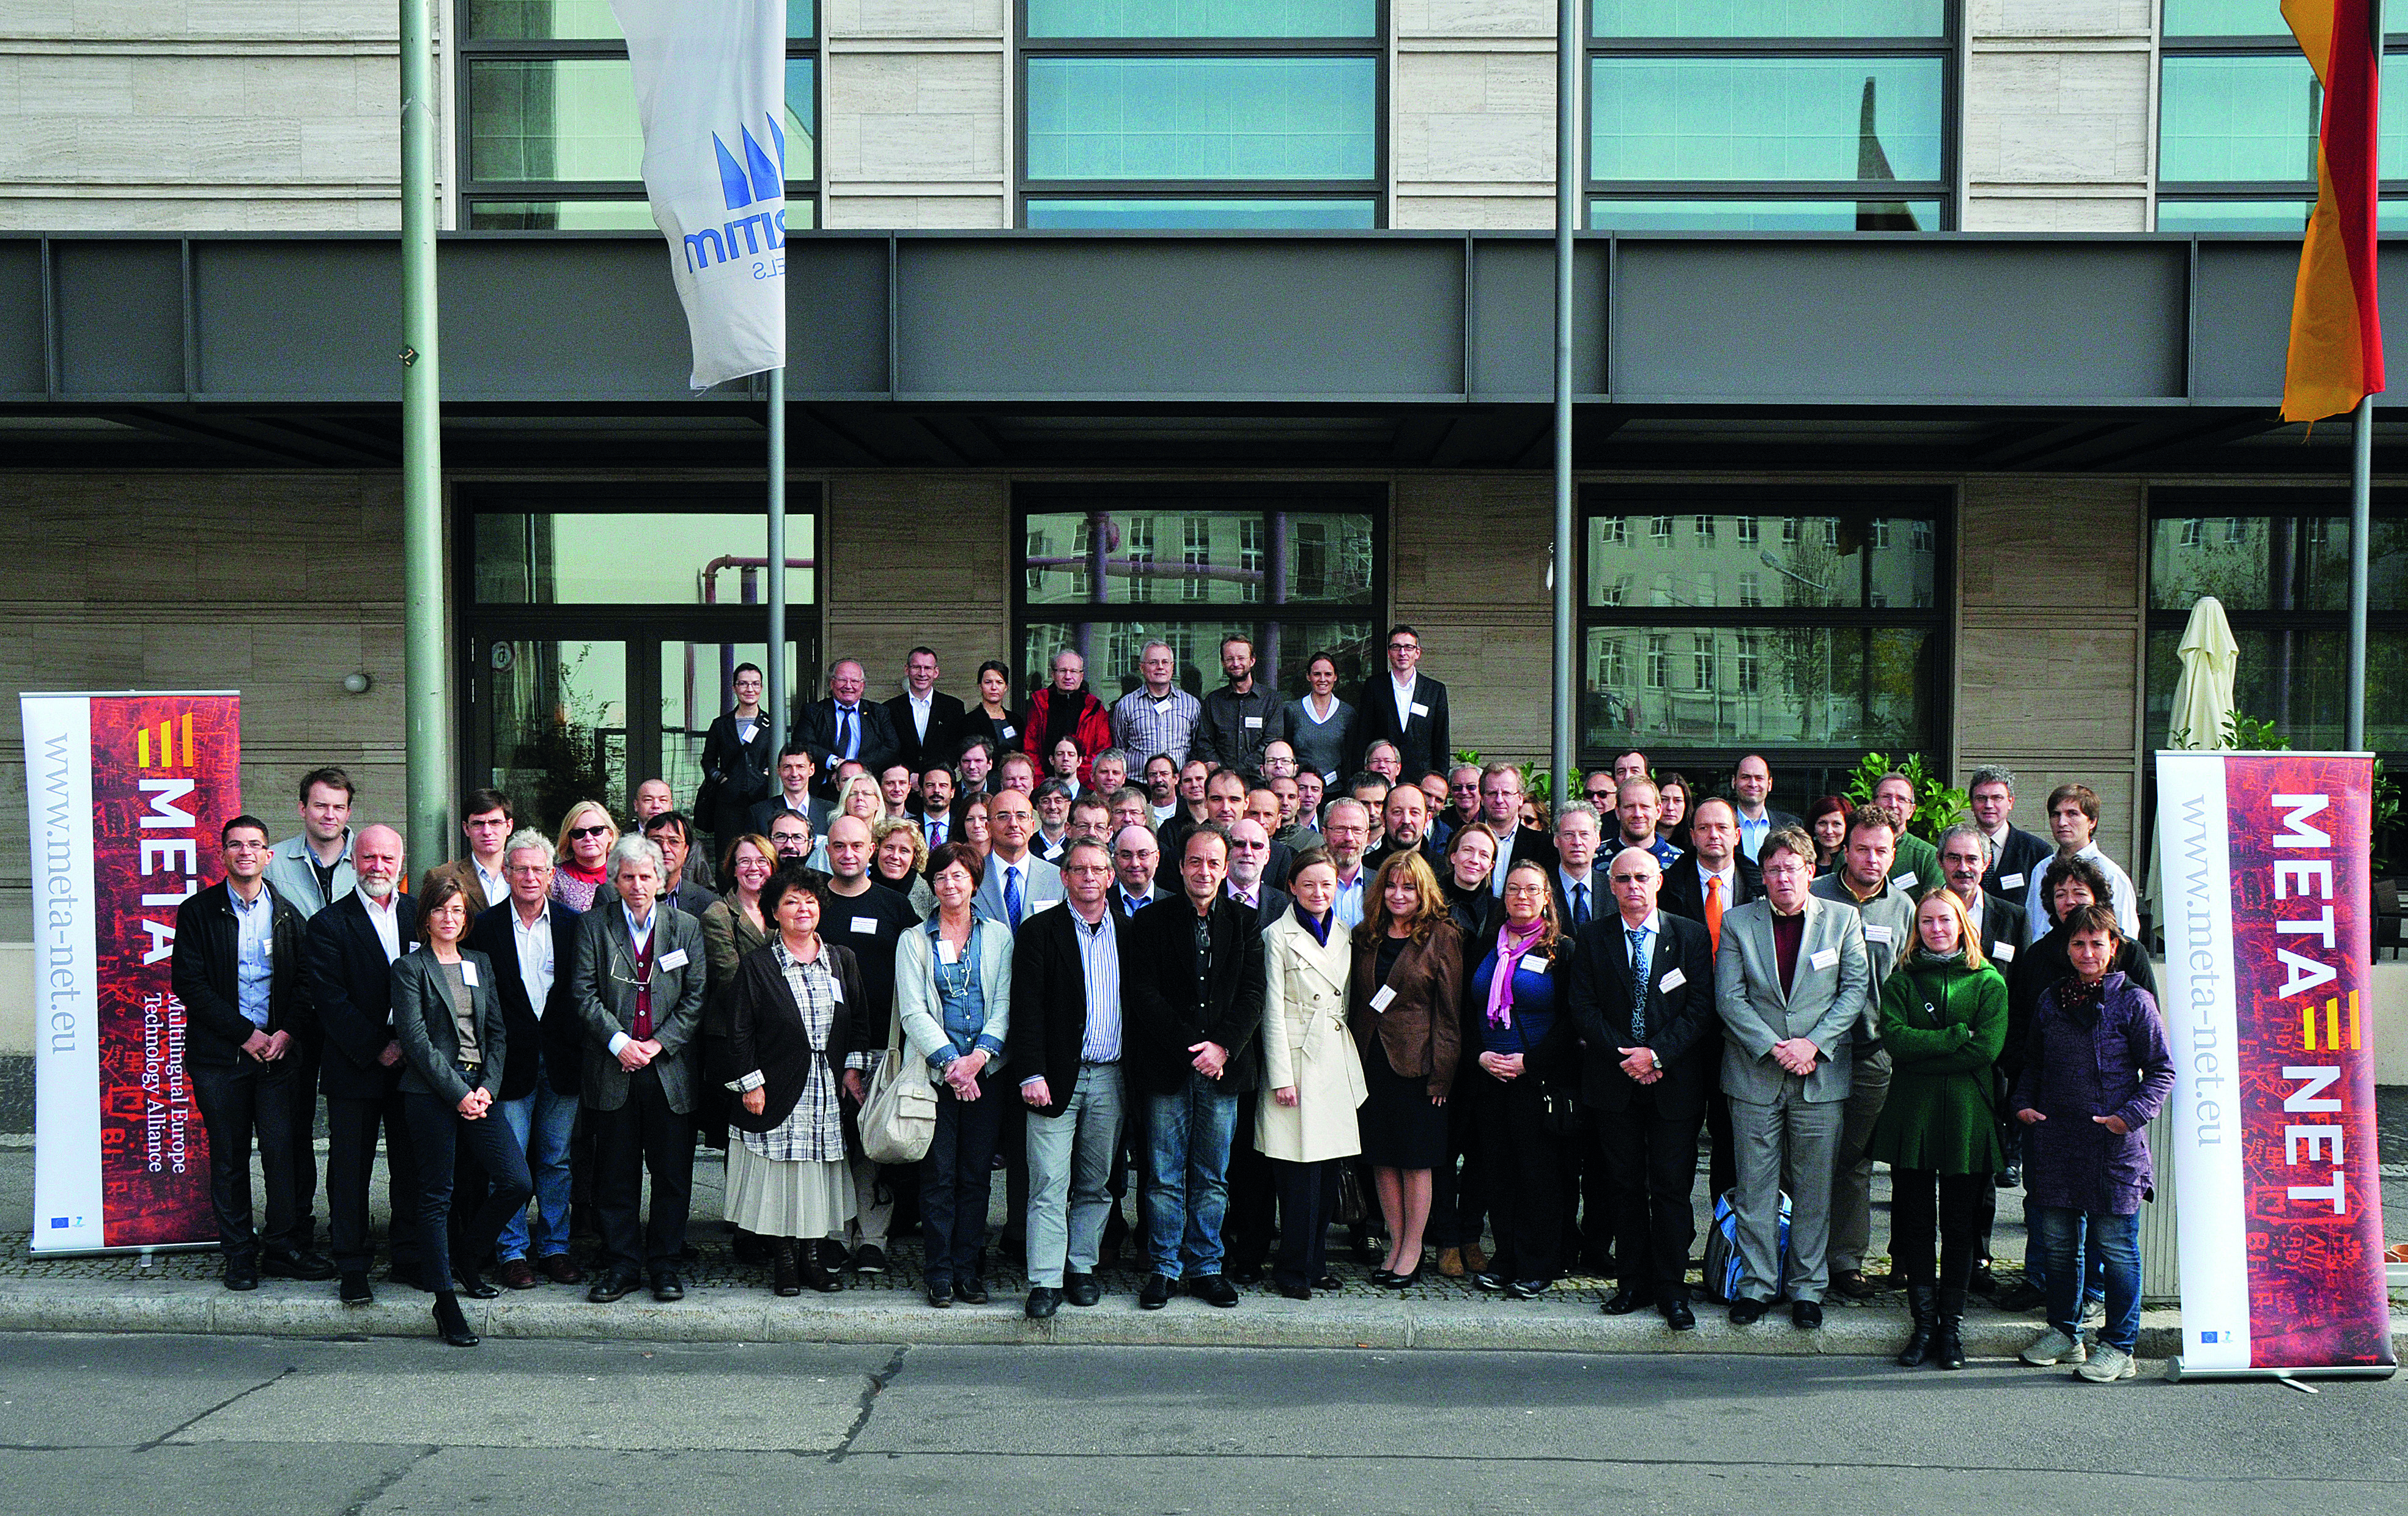
\includegraphics[width=\textwidth]{../_media/meta-net_team.jpg}
  \caption{About 100 language technology experts -- representatives of the countries and languages represented in META-NET -- discussed and finalised the key results and messages of the White Paper Series at a META-NET meeting in Berlin, Germany, on October 21/22, 2011.}
  \medskip
  \colorrule{grey3}{\textwidth}{1.5pt}
\end{figure*}

\cleardoublepage

\ssection[META Members]{META Members}
\label{metamembers}

% FIXME: Include a very tightly typeset list of the 630+ META members

\small
